\section{Experiments}

\subsection{Experimental conditions}\label{sec:results:data}

%\paragraph{Proteins.}
We consider two proteins: the $\beta$-galactosidase, a protein with a dihedral (D2) symmetry, and the lambda excision HJ intermediate (HJI), an asymmetric protein with local cyclic (C1) symmetriy. Both can be seen on \figref{pdb-proteins}.
Their deposited PDB atomic models are \texttt{5a1a}~\cite{bartesaghi2015betagal} and \texttt{5j0n}~\cite{laxmikanthan2016structure}, respectively.
For each atomic model, we generate the ground truth by fitting a 5\AA\ density map in Chimera~\cite{pettersen2004ucsf}.
We thus obtain a volume of $110 \times 155 \times 199$ voxels for the $\beta$-galactosidase, and a volume of $69 \times 57 \times 75$ voxels for the HJI.

\begin{figure}[ht!]
    \centering
    \begin{subfigure}[b]{0.45\textwidth}
        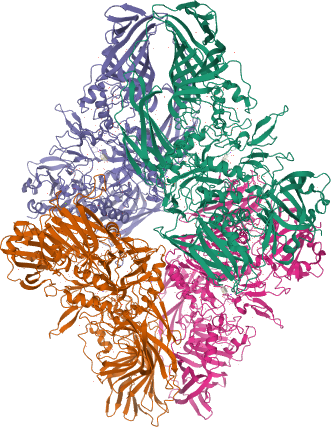
\includegraphics[height=5.5cm]{figures/5a1a_pdb.png}
        \caption{}
    \end{subfigure}
    %\hfill
    \begin{subfigure}[b]{0.45\textwidth}
    \centering
        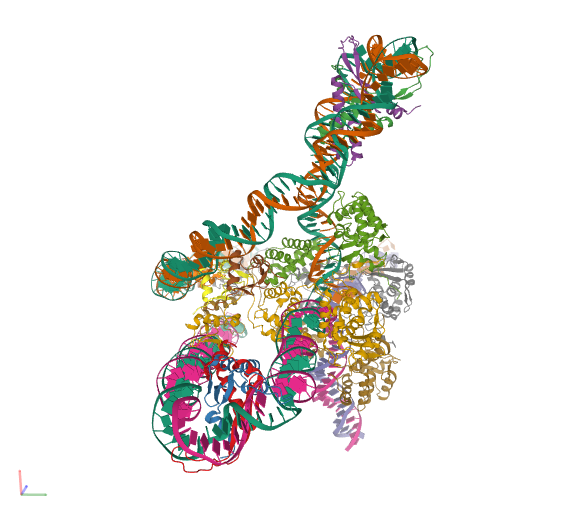
\includegraphics[height=5.5cm]{figures/5j0n_pdb.png}
        \caption{}
    \end{subfigure}

    \caption{%
        The two proteins we are working with.
        \textbf{(a)} $\beta$-galactosidase (\texttt{5a1a})~\cite{5a1a_pdb}.
        \textbf{(b)} lambda excision HJ intermediate (HJI) (\texttt{5j0n})~\cite{5j0n_pdb}.
    }\label{fig:pdb-proteins}
\end{figure}


\paragraph{Projections.}
From these ground truths, we generate $5,000$ synthetic projections of size $275\times 275$ and $116\times 116$, respectively, using the ASTRA projector~\cite{van2015astra}.
Our projection generator supports two orientation samplings: (i) sampling the Euler angles $\bth=(\theta_1,\theta_2,\theta_3)$ uniformly, and (ii) sampling uniformly on $\SO(3)$.
Due to protein symmetries, orientations are sampled differently.
For the entire \texttt{5j0n} complex is asymmetric~\cite{doi:10.1002/9780470514160.ch4}, thus it is sufficient to sample the \textit{half} of the $\mathbb{S}^2$ sphere, since the other half will have equivalent projections that are symmetric to the center of this sphere.
Conversely, the $\beta$-galactosidase has D2 symmetry, i.e., it is composed of four identical sub-units with two rotations of magnitude $\pi$ rad around the first axis followed by $\pi$ rad rotation around second axis, as illustrated and explained in~\cite{symmetry_in_protein,symmetry,scipion-em-github, rcsb-symmetry-view, EmpereurMot2019GeometricDO}.
Therefore, we restrict the sampling to the quarter of $\mathbb{S}^2$ sphere for this protein.
%\mdeff{We should explain why.}
\figref{different-projections} shows example projections.

\begin{figure}[ht!]
    \centering
    \begin{subfigure}[b]{0.3\textwidth}
        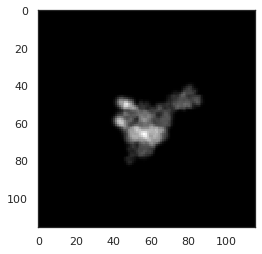
\includegraphics[height=4.8cm]{figures/5j0n_noise0}
        \caption{}
    \end{subfigure}
    \hfill
    \begin{subfigure}[b]{0.3\textwidth}
    \centering
        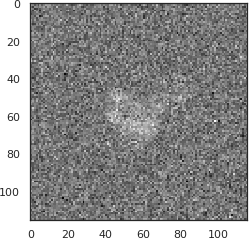
\includegraphics[height=4.8cm]{figures/5j0n_noise16}
        \caption{}
    \end{subfigure}
    \hfill
    \begin{subfigure}[b]{0.3\textwidth}
    \centering
        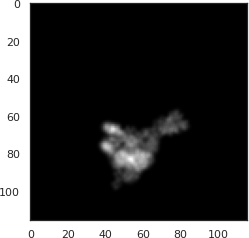
\includegraphics[height=4.8cm]{figures/5j0n_translated}
        \caption{}
    \end{subfigure}
    \caption{%
        An example projection being perturbed.
        \textbf{(a)} Unperturbed projection $\mathbf{P}_{\bth_i} \mathbf{x}$.
        \textbf{(b)} Perturbed projection $\mathbf{P}_{\bth_i} \mathbf{x} + \mathbf{n}$, with noise $\mathbf{n}$ sampled from a Gaussian distribution of mean 0 and variance 16.
        \textbf{(c)} Perturbed projection $\mathbf{S}_{\mathbf{t}} \mathbf{P}_{\bth_i} \mathbf{x}$, with translations $t_1$ and $t_2$ sampled from a triangular distribution with a lower limit of -20 pixels, an upper limit of 20, and a mode (i.e., peak) of 0.
    }\label{fig:different-projections}
\end{figure}

\paragraph{Perturbations.}
We consider the following perturbations to control the difficulty of orientation recovery: (i) additive white noise, (ii) translations, (iii) point-spread functions (PSF). Mathematical formulation of these three components is shown in \eqnref{imaging-model}.

\begin{table}[ht!]
    \centering
    \begin{tabular}{lrrr}
        \toprule
        Dataset & Number of projections $P$ (\%) & Maximum number of pairs $P^2$ & Used number of pairs \\
        \midrule
        Train & 2512 (50\%) & 6,312,656 & 63,126 (1\%) \\
        Validation & 1650 (33\%) & 2,722,500 & 27,225 (1\%) \\
        Test & 838 (17\%) & 701,406 & all (sampled per batch) \\
        \bottomrule
    \end{tabular}
    \caption{
        Split of $P=5000$ projections (for both \texttt{5j0n} and \texttt{5a1a}) in training, validation, and test sets.
    }\label{tab:dataset}
\end{table}

\paragraph{Distance learning.}
We use supervised learning, thus training on input-output pairs.
The input are two images and the output is their quaternion distance calculated from the ground truth orientations.
For the training, dataset is split into a distinct training, validation, and testing set (see \tabref{dataset}).
The total number of generated projections is $P = 5,000$.
Therefore, the number of possible projection pairs is $P^2 = 25e6$.
Splitting $P^2$ into the training, validation, and testing sets would mean that some of the projections appearing in pairs in the training dataset can appear in pairs in the other datasets.
To ensure that the results generalize to unseen data, we split the projections $P$ (and not $P^2$) into training, validation, and testing projection sets.
With these three projections sets we create disjoint projection pair datasets sets (column with $P^2$ values in \tabref{dataset}).
In addition to this, we use only $1\%$ of the possible pairs (last column in the \tabref{dataset}) due to limitation of available resources for the training.
%\todo{Better explain why projections (and not pairs) must be separated in the various sets.}


\paragraph{Orientation recovery.}
Orientations are recovered through \eqnref{orientation-recovery} and it was done in a stochastic setting, where the loss function varies over the batches.
Hence, the dataset used in this part is test set from \tabref{dataset}.
Orientation recovery is performed on projections unseen during distance learning.

\figref{5j0n-aa-loss-perfect-distances} shows a successful convergence and mean orientation recovery error before and after alignment with the perfect distance $d_q$.
There many different ways of evaluating the pipeline performance found in the field of pose estimation. Some of the evaluations include the following:
\mdeff{Shall we keep this? Not as a bullet list for sure.} \lau{Maybe in the Appendix, but not in the main text imo.}
\begin{itemize}
\item Intersection over Union (IoU) of the object 3D cloud with a custom threshold classifying it as a good estimate or not (e.g. in the paper~\cite{10.1007/s11263-014-0733-5} the threshold score above 0.5 is considered good estimation).
\item Translation and rotation error between estimated 3D model and true 3D model with fixed thresholds (e.g. in the paper~\cite{shotton2013scene} they require the translation error to be below 5 cm and rotation error to be below 5\degree)
\item The average distance of all the points of the model from their transformed version, and if the error is less than the constant multiple of diameter of the 3D model, it is considered correctly evaluated (e.g. evaluation error is used in papers \cite{10.1007/978-3-642-37331-2_42, xiang2018posecnn})
\item Reprojection error that projects the estimated points onto the image and computes the pairwise distances in the image space, instead of computing distances in the 3D model space (e.g. used in paper~\cite{xiang2018posecnn})
\item The recovery error measured as Frobenius norm from estimated 3D model and true model, where 3D model is composed of 3D locations of important landmarks (e.g. elbow for human pose estimation)~\cite{wangni2018monocular}
\item Average Orientation Similarity (AOS) is the difference between the true and estimated model with a cosine similarity term~\cite{RedondoCabrera2016PoseEE}
\item Mean Angle Error (MAE) and Median Angle Error (MedError) evaluated and compared with other pose estimation error metrics in the paper~\cite{RedondoCabrera2016PoseEE}.
\end{itemize}
Since mean orientation error is used in the pose estimation tasks and it is considered reliable performance metric, we decided to use it as our performance measure. We employ the definition of a correct estimation: the estimation must be within 10\degree~(0.174 rad) of true orientations for noiseless data and within 25\degree~(0.436 rad) for noisy data.

%\mdeff{Why is it good? Intuitive sure. Laurène, can we say something more?}

%%%%%%%%%%%%%%%%%%%%%%%%%%%%%%%%%%%%%%%%%%%%%%%%%%%%%%%%%%%%%%%%%%%%%%%%%%%%%%%%%%%%%%%
\subsection{Results}\label{sec:results:orientation-recovery}

To evaluate our method, we start with the orientation recovery experiments that include tests of feasibility and sensitivity to distance estimation error. Then we learn the distance using a SiameseNN and compare its performance with the baseline. After developing and tuning the architecture of the network for the distance estimation, we continue by introducing the perturbation to the projections. Finally, we run the whole machine learning pipeline to recover the orientations from estimated distances.

%\mdeff{Story: good distance estimation = good orientation recovery.}
% \begin{algorithm}[H]
% \SetAlgoLined
% \KwResult{Write here the result }
%  initialization\;
%  \For{$steps \gets 1$ \textbf{to} $30000$}{
%   instructions\;
%   \eIf{condition}{
%   instructions1\;
%   instructions2\;
%   }{
%   instructions3\;
%   }
%  }
%  \caption{Orientation recovery algorithm}
% \end{algorithm}


%\subsubsection{Robustness of Recovery to Additive Errors on the Relative Distances}
\subsubsection*{Orientation recovery: Sensitivity to distance estimation error}\label{sec:results:orientation-recovery:sensitivity}

%\mdeff{Story: (i) orientation recovery error is strongly linked to distance estimation error, (ii) recovery loss is a good proxy of mean recovery error.}

To prove the the orientation recovery is feasible, we first evaluate the performance assuming we have ideal distance metric between two projections, i.e., the quaternion distance between their corresponding orientations. The method successfully recovers the orientation of every projection, see Appendix~\ref{apx:results:orientation-recovery:exact}.

We now go one step further and evaluate the behaviour of~\eqnref{orientation-recovery} when the true relative distances are corrupted by additive Gaussian noise.

The experimental conditions are the same as in the previous section, except that we add an error with increasing variance on the relative distances prior to the minimization. Precisely: $d_p = d_q + n$ with $n$ sampled from a Gaussian distribution with mean 0 and variances in $[0.0, 0.8]$.
The results are presented in \figref{perfect-with-noise-ar-aa} (red curve).
For all variances, the mean orientation recovery error $E$ is reported in \figref{perfect-with-noise-ar-aa} (blue curve).

\begin{figure}[ht!]
    \centering
    \begin{subfigure}[b]{0.48\textwidth}
        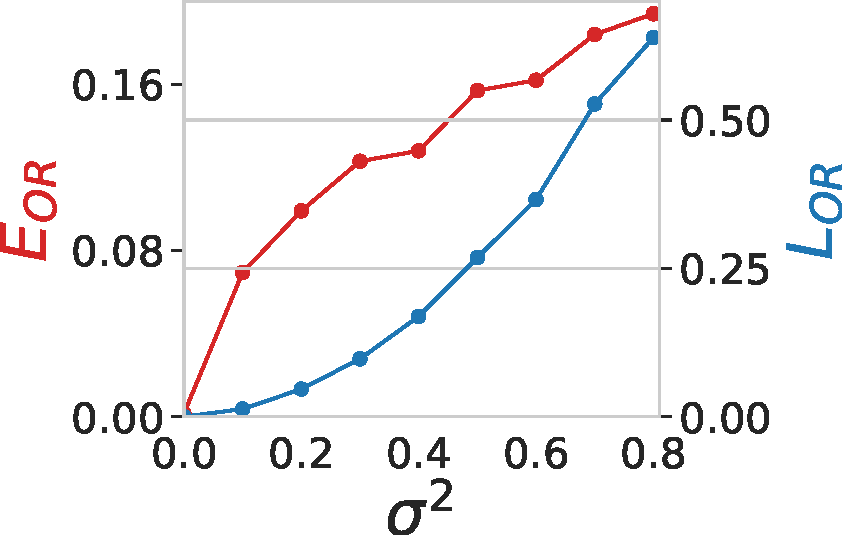
\includegraphics[height=5.5cm]{figures/5j0n_perfect_noisy_ar_aa}
        \caption{Asymmetric protein (\texttt{5j0n}).}
    \end{subfigure}
    \hfill
    \begin{subfigure}[b]{0.50\textwidth}
    \centering
        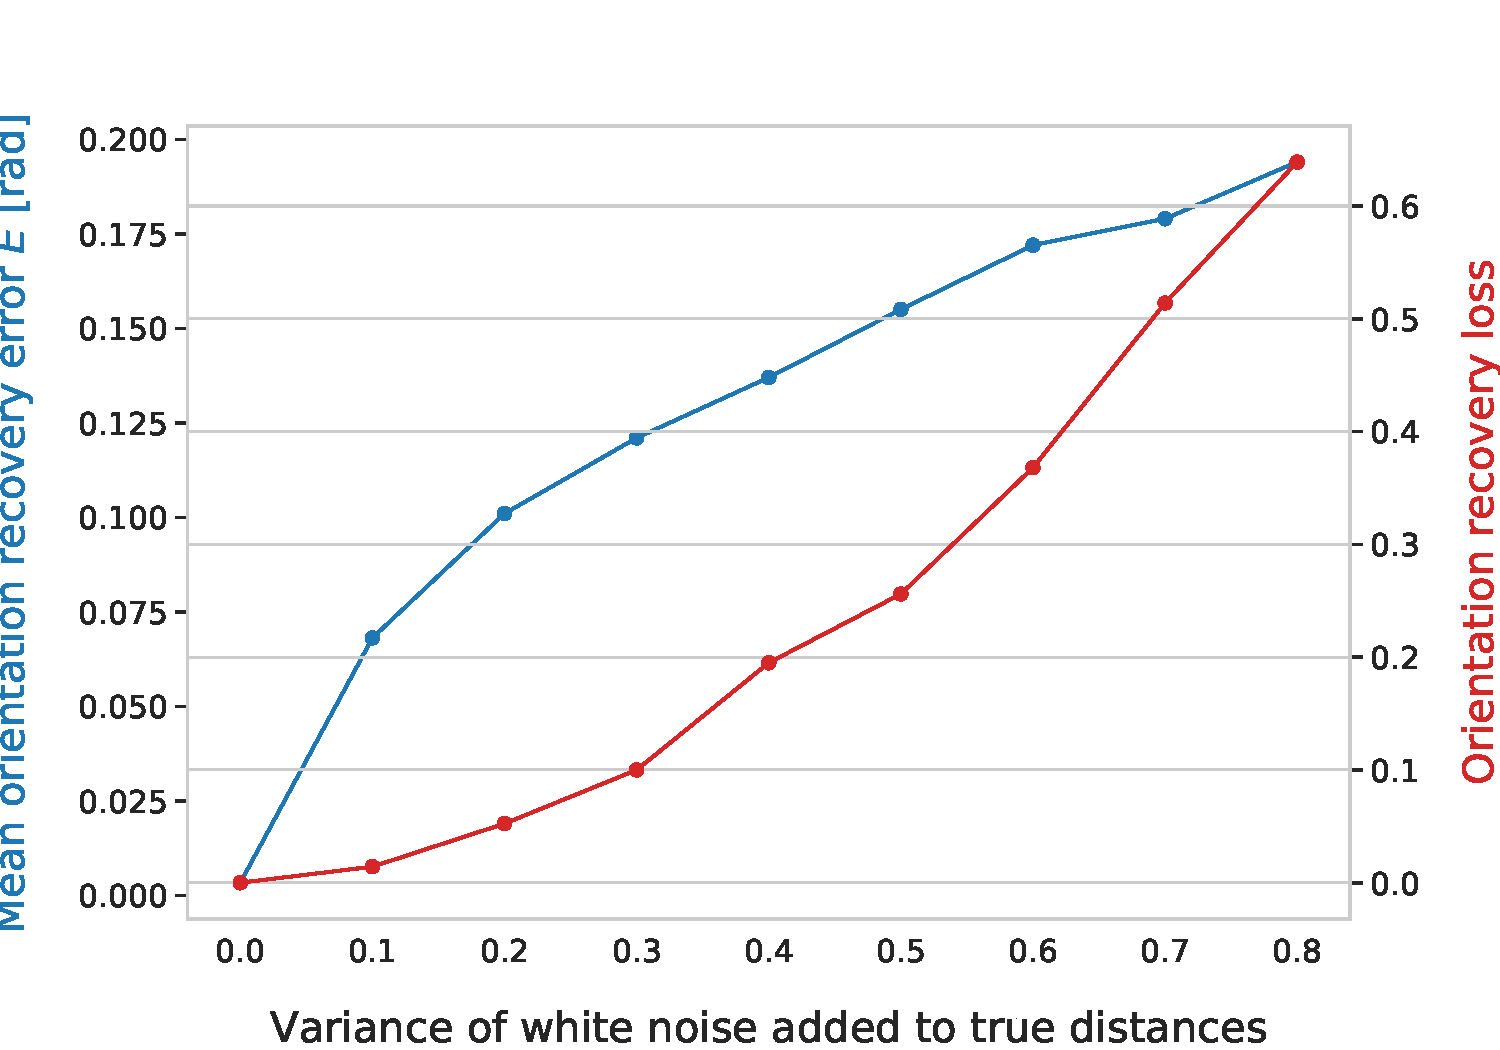
\includegraphics[height=5.5cm]{figures/5a1a_perfect_noisy_ar_aa}
        \caption{Symmetric protein (\texttt{5a1a}).}
    \end{subfigure}
    \caption{
        The mean orientation recovery error $E$ from \eqnref{orientation-recovery-error} is a monotonic function of the distance estimation error.
        Better distance estimation leads to better orientation recovery.
        Moreover, the recovery loss \eqnref{orientation-recovery} is a good proxy for the recovery error $E$, allowing us to assess recovery performance even without ground-truth orientations.
}
    \label{fig:perfect-with-noise-ar-aa}
\end{figure}

These results demonstrate that the performance of orientation recovery~\eqnref{orientation-recovery} depends on the quality of the estimated distances, which advocates for a proper and extensive training of the SiameseNN in the next stages of development.
Another interesting output of \figref{perfect-with-noise-ar-aa} is that it indicates that the error of the orientation recovery behaves as a monotonic function of its loss.
Hence, it suggests that the loss can be used as a good indicator of its performance, which has obvious practical implications for our future works on real data.

%%%%%%%%%%%%%%%%%%%%%%%%%%%%%%%%%%%%%%%%%%%%%%%%%%%%%%%%%%%%%%%%%%%%%%%%%%%%%%%%%%%%%%%


\subsubsection*{Distance estimation: Learned distance}\label{sec:results:distance-estimation:learned}

%\mdeff{Story: learned distance $d_{ps}$ estimates $d_q$ with some variance but still underestimates larger distances.
%Again symmetric vs asymmetric.}

We present here a preliminary evaluation of the ability of SiameseNNs to learn a projection distance $\widehat{d_p}$ that correctly approximates the orientation distance $d_q$. To asses the progress and effectiveness of our distance estimation implementation, we used an Euclidean distance as a baseline, see Appendix~\ref{apx:results:distance-estimation}.

%SiameseNNs come with a variety of more or less powerful architectures.
%At the current stage of development, we work with a simple one.
%Our SiameseNN is composed of two convolutional neural networks (CNNs) with shared weights.
%Their output features vectors are compared through an Eulidean distance, \textit{i.e.}, $d_f(\mathbf{f}_i,\mathbf{f}_j)=\lVert \mathbf{f}_i-\mathbf{f_j}\rVert_2$ in \figref{schematic:distance-learning}.
%Besides the Euclidean distance, this distance metric $F$ can be defined as geodesic distance, or it could be parametrized as MLP, used for a general function approximation, which we will explore in some of the following experiments.
%\mdeff{Don't repeat what's written in \secref{method:distance-learning}. The general stuff goes there, the specific here.}

\begin{figure}
    \centering
    \begin{subfigure}[t]{0.45\textwidth}
        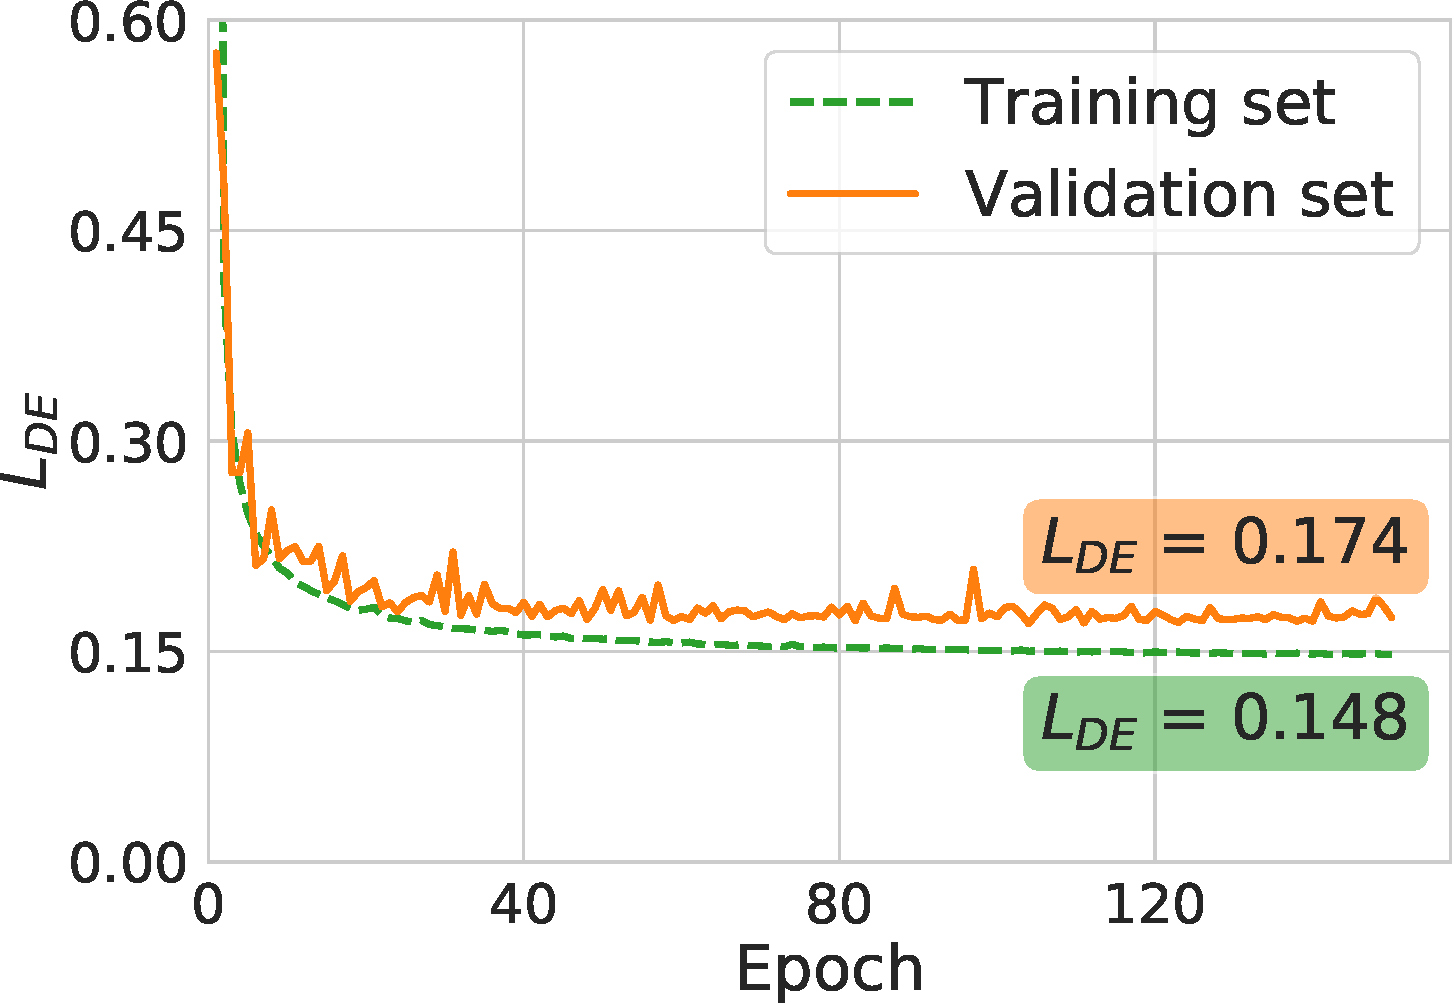
\includegraphics[height=6cm]{figures/de_5j0n}
        \caption{Asymmetric protein (\texttt{5j0n}).}
        \label{fig:losses-siamese-assym}
    \end{subfigure} \quad \quad
    \begin{subfigure}[t]{0.5\textwidth}
        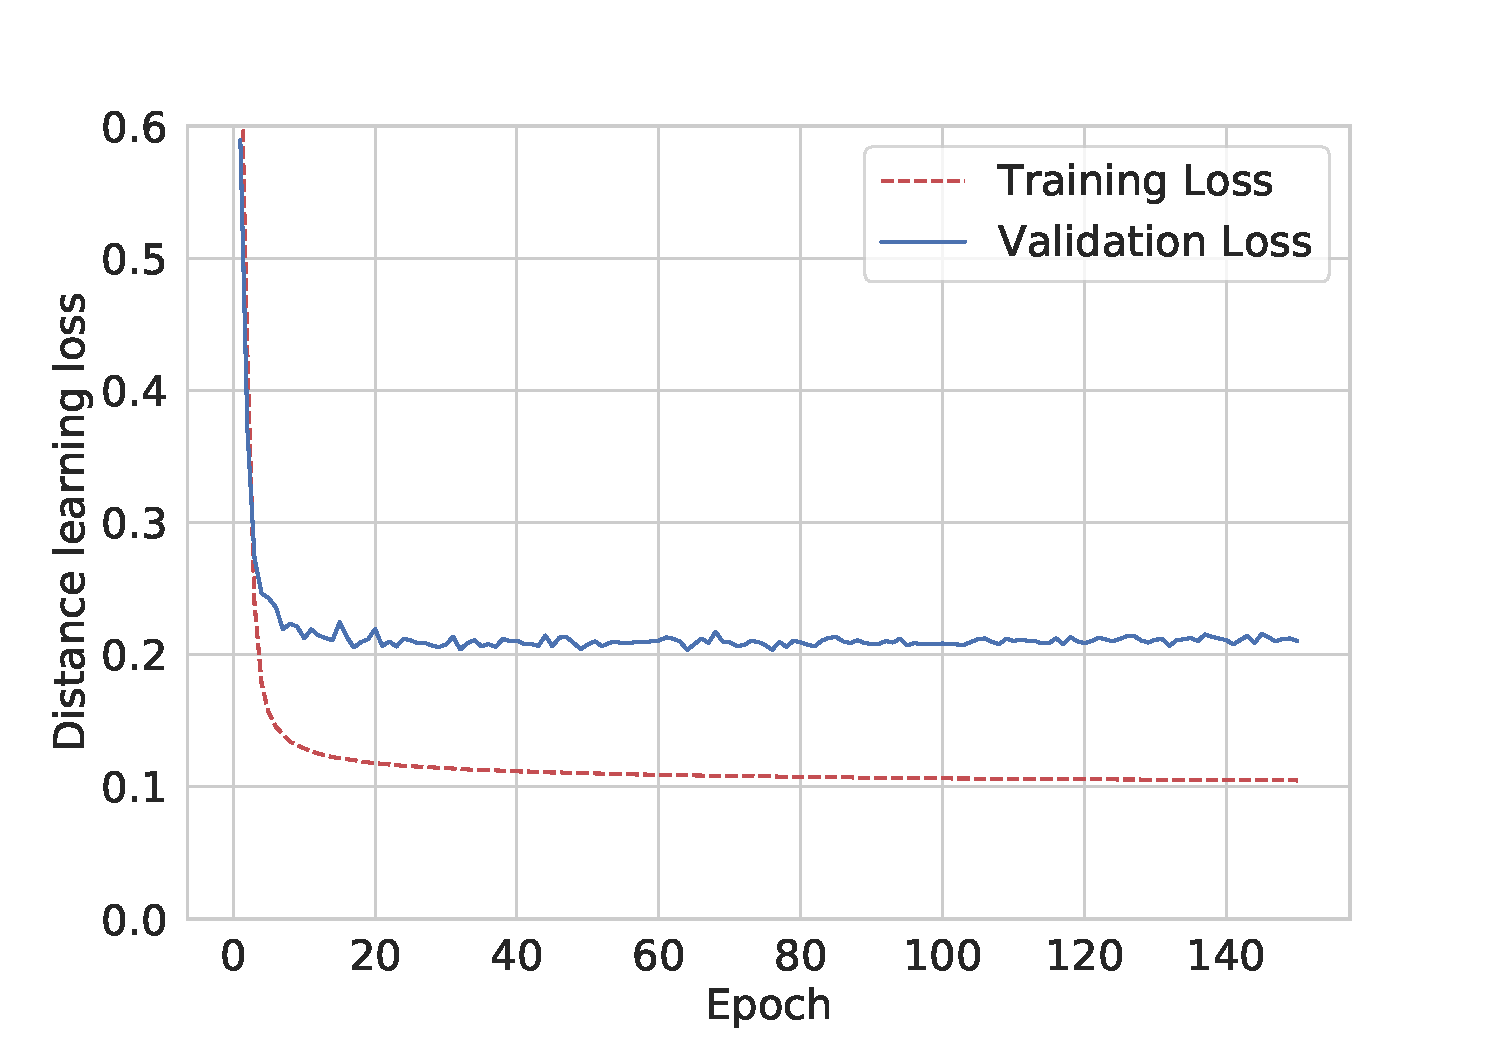
\includegraphics[height=6cm]{figures/de_5a1a}
        \caption{Symmetric protein (\texttt{5a1a}).}
        \label{fig:losses-siamese-sym}
    \end{subfigure}
    \caption{
        Distance learning loss \eqnref{distance-learning} evaluated on the training and validation datasets during learning/training.
    }\label{fig:losses-siamese}
\end{figure}

\begin{figure}
    \centering
    \begin{subfigure}[b]{0.5\columnwidth}
        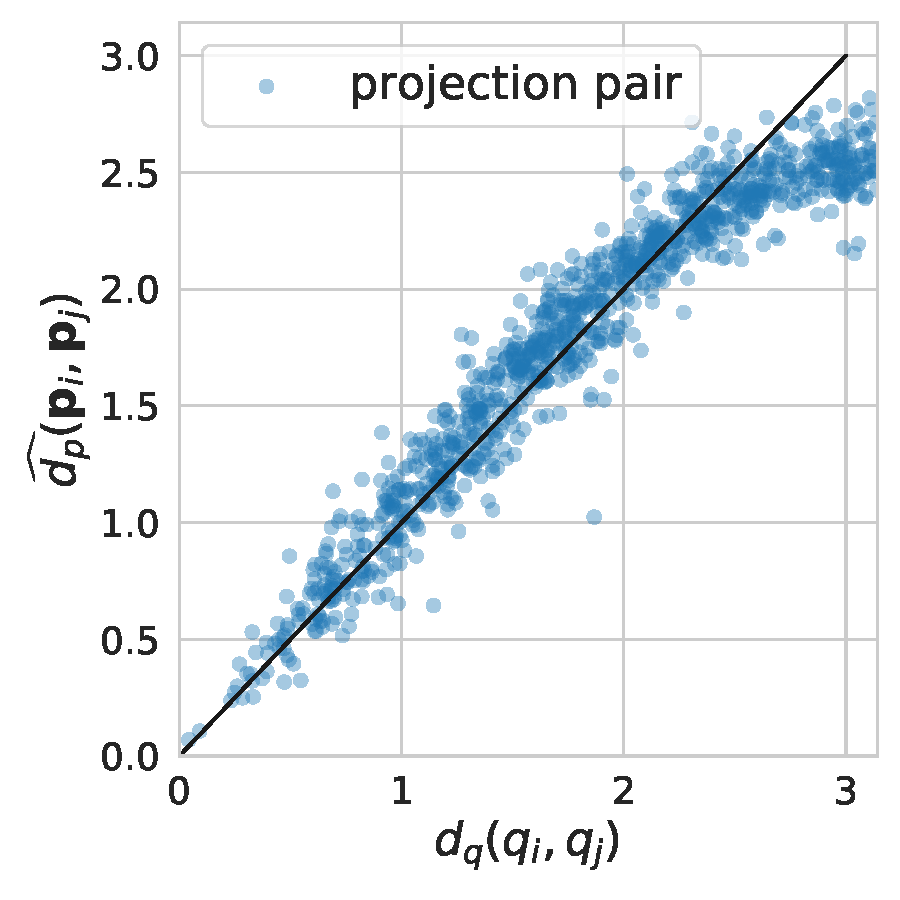
\includegraphics[height=6cm]{figures/dPdQ_5j0n}
        \caption{Asymmetric protein (\texttt{5j0n}) on test dataset.}
    \end{subfigure}
    %\hfill
    \begin{subfigure}[b]{0.45\columnwidth}
    \centering
        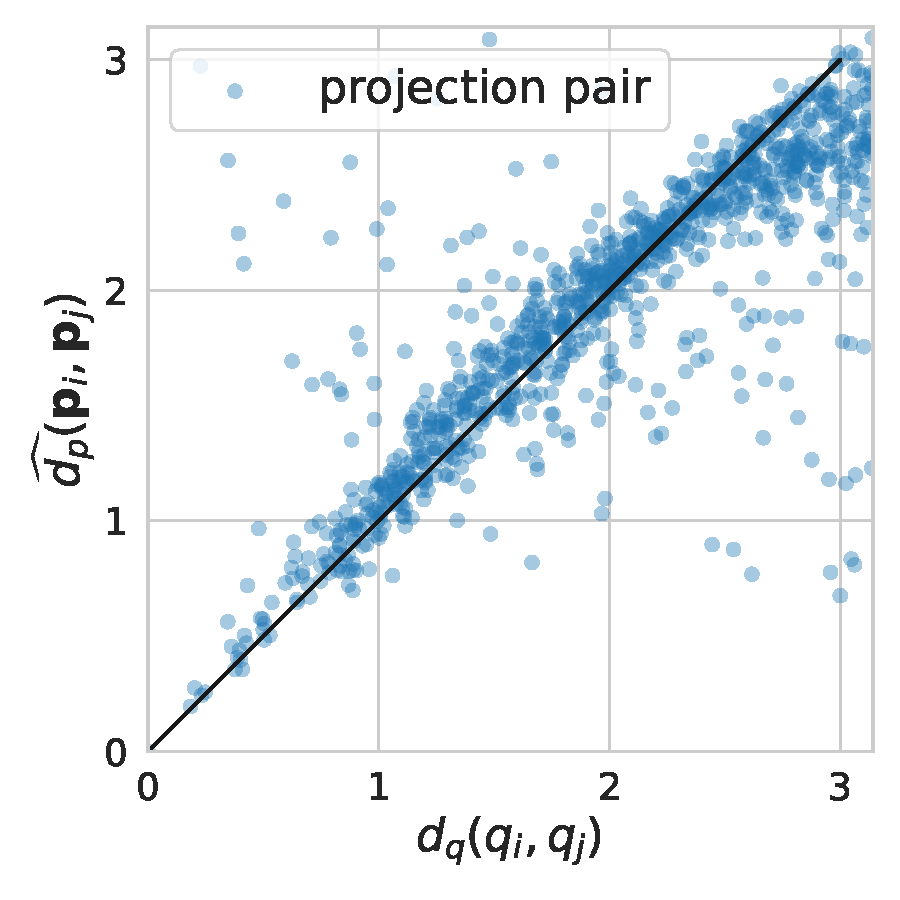
\includegraphics[height=6cm]{figures/dPdQ_5a1a}
        \caption{Symmetric protein (\texttt{5a1a}) on test dataset.}
    \end{subfigure}
    \caption{Relationship between orientations' distance $d_q$ and estimated distance $d_p$.}
    \label{fig:learned-distance-siamese}
\end{figure}

%\mdeff{What is $d_f$ in this particular experiment? Euclidean? Cosine=$d_q$?}
For each protein, we train the SiameseNN on its training dataset for 150 epochs ($\sim$2.6 hours) using an RMSProp optimizer~\cite{tieleman2012rmsprop}, a learning rate of $10^{-3}$, and a batch size of 256 pairs. As a feature distance $d_f$ between the outputs of the two CNNs we use the Geodesic distance \eqnref{geodesic-distance}.
The pairs for the training are sampled from $1\%$ of maximum number of training pairs $P_{\text{train}}^2$ ($63,126$ pairs) and validation is performed on $1\%$ of the maximum number of validation pairs $P_{\text{val}}^2$ ($27,225$ pairs). We limit our training and validation dataset due to Google Colab training time limit of 12 hours.

%\mdeff{So those pairs are sampled from $63,126$ pairs from the training dataset, rather than the $P^2$ possible pairs? If true, we should motivate somewhere why we limit our training dataset.}
Depending on the available resources on the Google Colab, the training can last from 2.6 hours to 9.3 hours on one of its GPUs.
The evolution of the training and validation losses are presented in \figref{losses-siamese-assym} for the asymmetric protein (\texttt{5j0n}), and in \figref{losses-siamese-sym} for the symmetric one (\texttt{5a1a}).
The results demonstrate that the SiameseNN succeeds at learning a proxy distance for the asymmetric protein dataset, as convergence is reached in about 50 epochs ($\sim$ 50 minutes in the best resource availability setting).

%\todo{Mention the plateau phenomenon, similarly to Euclidean $d_p$.}
Similarly to Euclidean distance $d_p$, we notice that the larger distances $d_q$ are poorly predicted and the plot again has a slight plateau phenomenon for the distances higher than ~$2.5$ rad.

It is interesting that both validation losses are around $0.2$.
However, the current SiameseNN architecture slightly overfits at learning the distance for the dataset \texttt{5a1a}, which is very likely due to the symmetry of the $\beta$-galactosidase protein, even thought the quarter-sphere coverage was used.
%Indeed, its synthetic dataset may still contain pairs of projections that share the same $d_p$, yet differ in their $d_q$.
This simply advocates for the restriction to non-overlapping areas on $\SO(3)$ when sampling the orientations used to generate the SiameseNN training dataset.
The latter would then only contain projection pairs with a linear $(d_q,d_p)$ relationship, which should ensure a successful training of the network.
%\mdeff{I don't get this explanation. Do you mean that \texttt{5a1a} might have other symmetries than D2?}
For the rest of the experiments, we use the asymmetric protein (\texttt{5j0n}) dataset.
Besides using the asymmetric protein, we will perform the full protein reconstruction pipeline on the symmetric protein (\texttt{5a1a}).

We then feed to the trained SiameseNN $1,000$ pairs of projections randomly selected from the \texttt{5j0n} testing dataset, and report the $(d_q,\widehat{d_p})$ relationship of each pair in \figref{learned-distance-siamese}.
These results confirm that, the SiameseNN is able to predict the orientation distance $d_q$ using only the projections as inputs. The prediction performance is slightly better for the asymmetric protein compared to symmetric protein.
Moreover, it clearly outperforms the Euclidean distance at doing so.
These preliminary results are encouraging, as much has yet to be gained from improving upon the rather primitive SiameseNN architecture we currently use. The architecture of implemented SiameseNN can be seen in Appendix~\ref{sec:siamese-architecture}. Besides concentrating on the hyperparameter selection and tuning of the neural network layers, we also evaluated the performance of the model depending on the feature distance we used for the SiameseNN, see\figref{geo-eucl-mlp} and Appendix~\ref{apx:de-influence-arch}.



\subsubsection*{Distance estimation: Sensitivity to perturbed projections}\label{sec:results:distance-estimation:sensitivity}

%\mdeff{Story: learned distance is minimally sensible to perturbations (additive noise, translation, PSF) because we can train it to ignore irrelevant information.
%Thanks again to good model of cryo-EM imaging.}
%\mdeff{Better word? (perturbations, quality, non-ideal)}

In this experiment we want to explore how does the perturbation of the projections affect the distance estimation (additive noise, translation, PSF).

The experimental conditions for the experiment are the same as before, except that we add noise with increasing variance on the projection prior to training.
The results are presented in \figref{distance-estimation-vary-projection-noise}.

We observe that the training and validation losses are increasing and network starts to overfit w.r.t.\ the amount of noise in the projections.
With the noiseless projections (projection noise variance 0), the mean orientation recovery error $E = 0.1594$ rad.
Whereas, the noisy projections with noise levels 15 are the closest to the realistic protein projections and the error $E=0.4189$ rad.
The SiameseNN is able to learn the noise as the training loss and corresponding mean orientation recovery error $E$ stays low.
%\mdeff{The SiameseNN seems to be able to learn the noise, as the training loss stays low. More data should help!}

Besides testing the performance of the pipeline with the noisy projections, we explore the performance with different projection translation levels.
To translate the projection, we use a triangular distribution from $-t$ to $t$ px translation with the peak in the center of the projection.
The performance of different translation magnitudes can be seen in \figref{distance-estimation-vary-projection-translation}.
We observe that the training of the network is invariant to translations in the projections, which was expected.
%\mdeff{Perfect!}

We can see that the learned distance is minimally sensible to perturbations because we can train the network to ignore irrelevant information.


\begin{figure}[ht!]
    \centering
    \begin{subfigure}[b]{0.47\textwidth}
        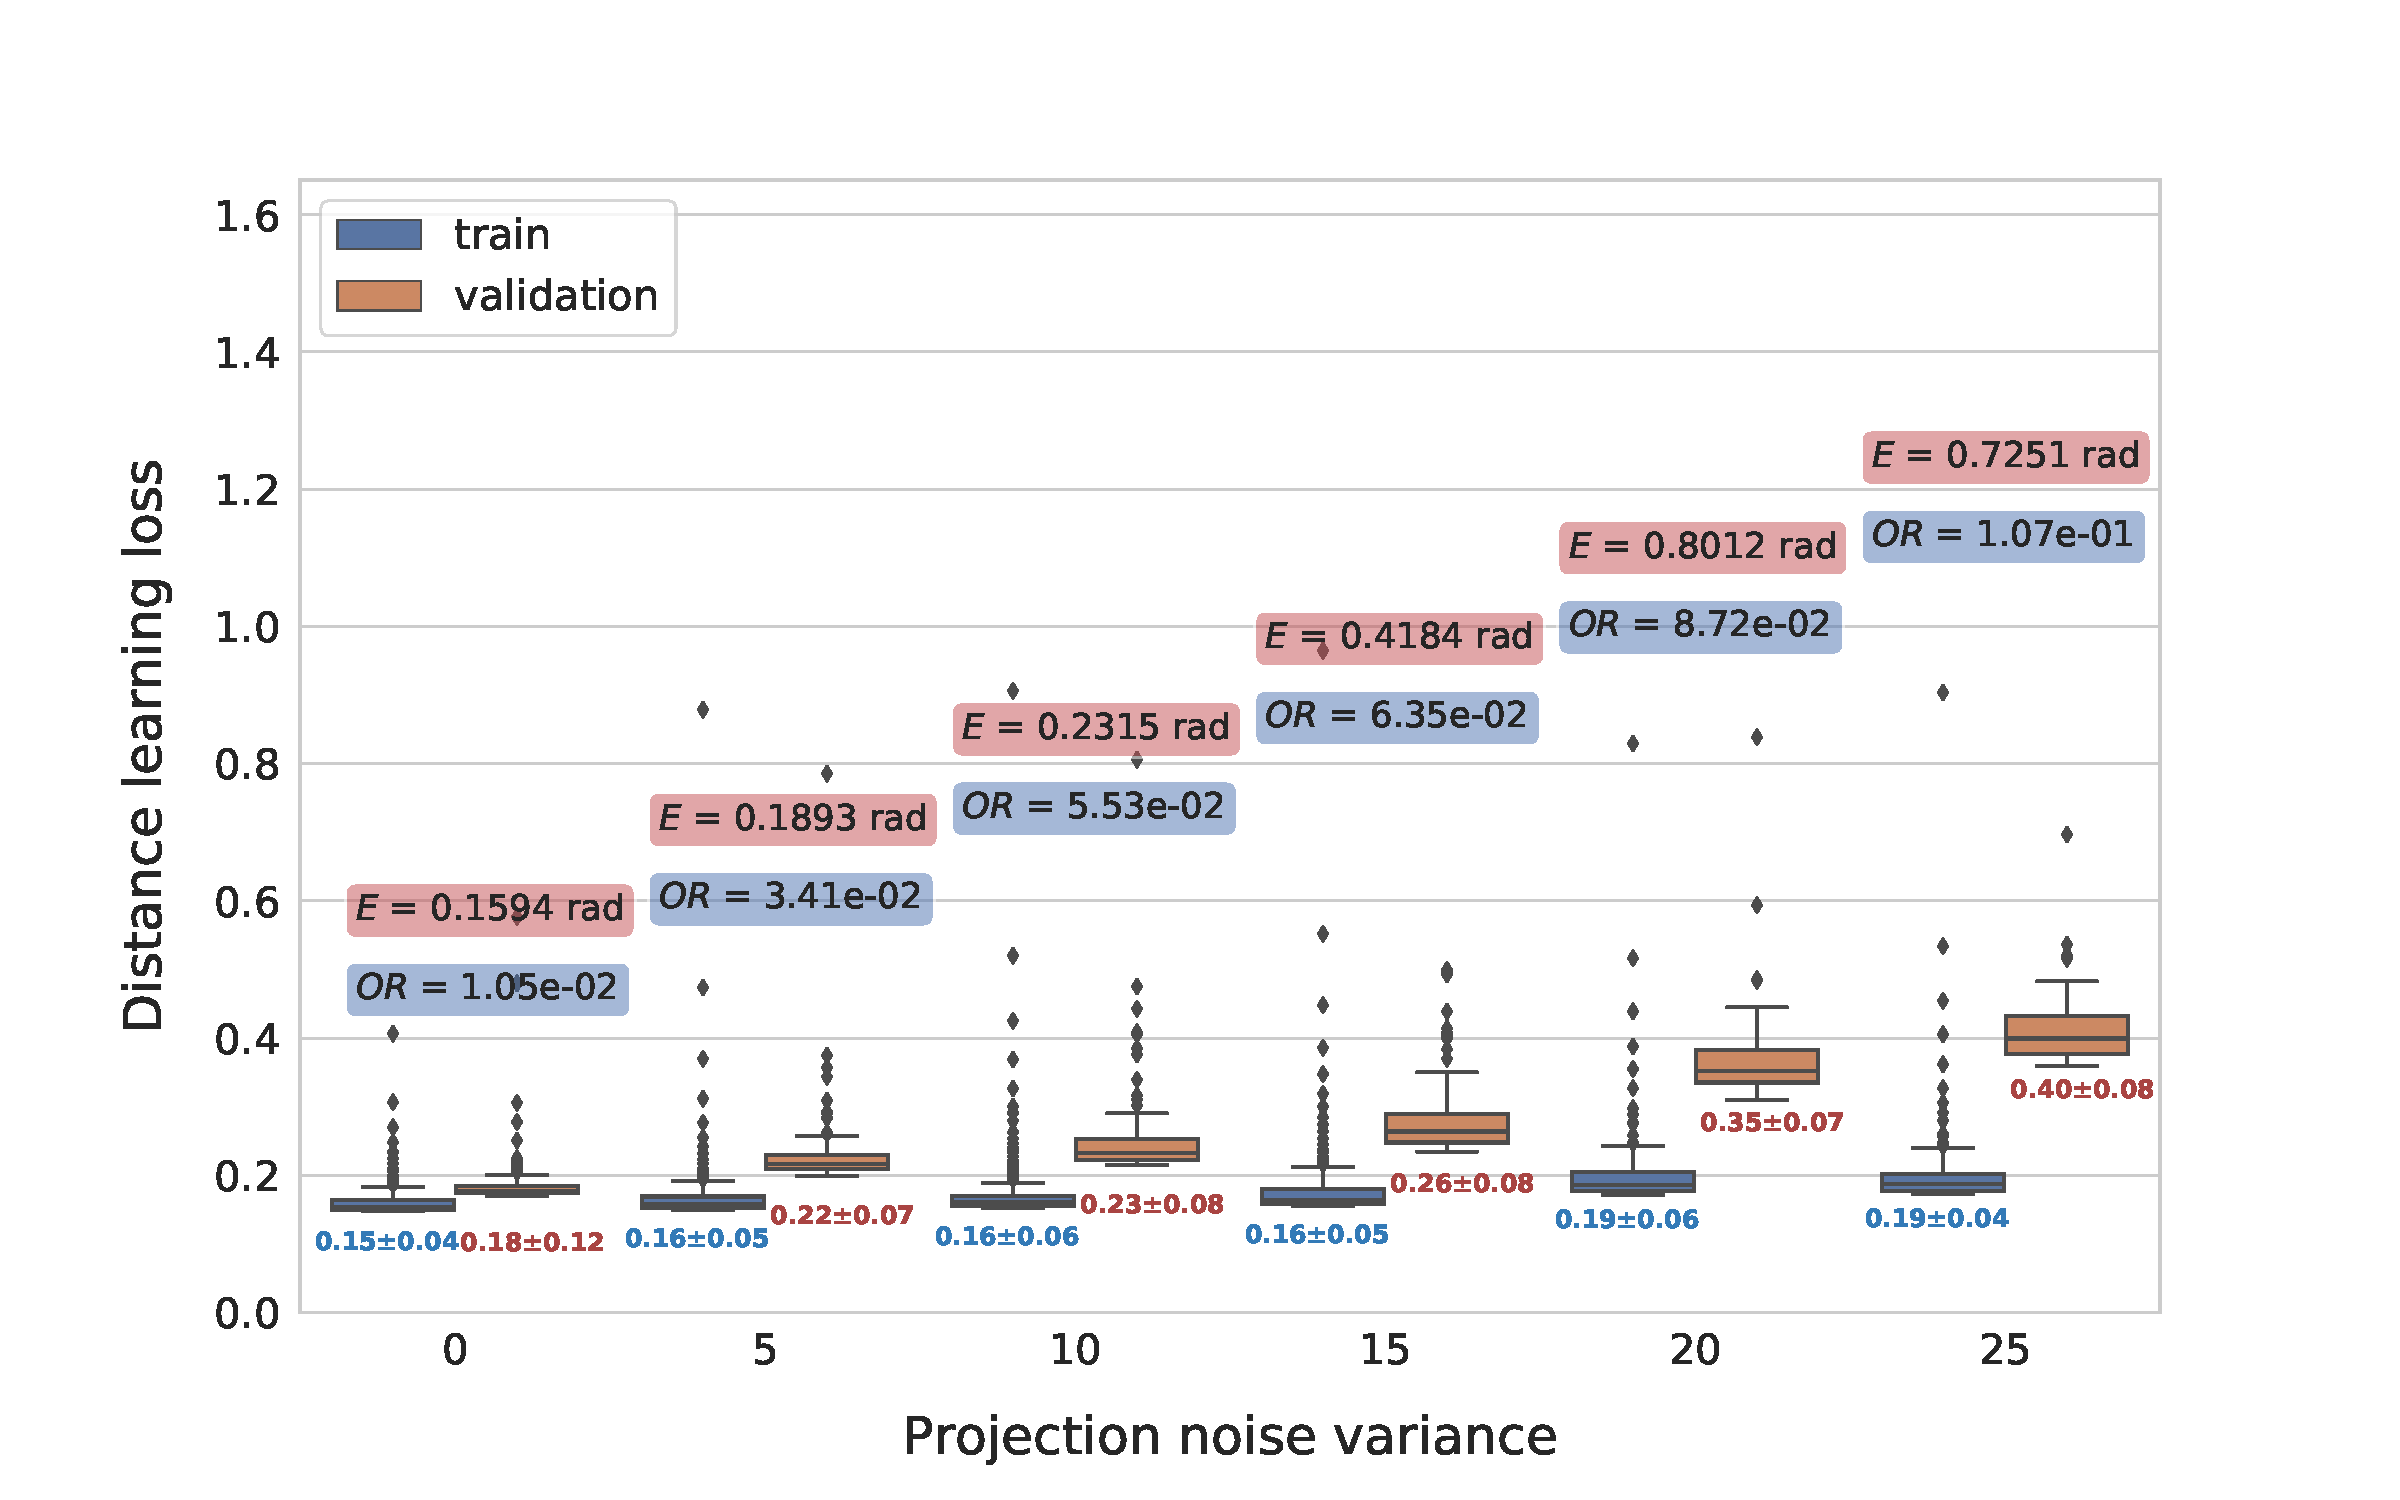
\includegraphics[height=5.5cm,valign=t]{figures/de_noises_nums}
        \caption{%
            Variation of train and validation epoch losses w.r.t. noise levels in the projections of the asymmetric protein (\texttt{5j0n}). The mean orientation recovery error $E$ is in the red box, and the orientation recovery loss $OR$ is in the blue box.
        }\label{fig:distance-estimation-vary-projection-noise}
    \end{subfigure}
    \hfill
    \begin{subfigure}[b]{0.47\textwidth}
        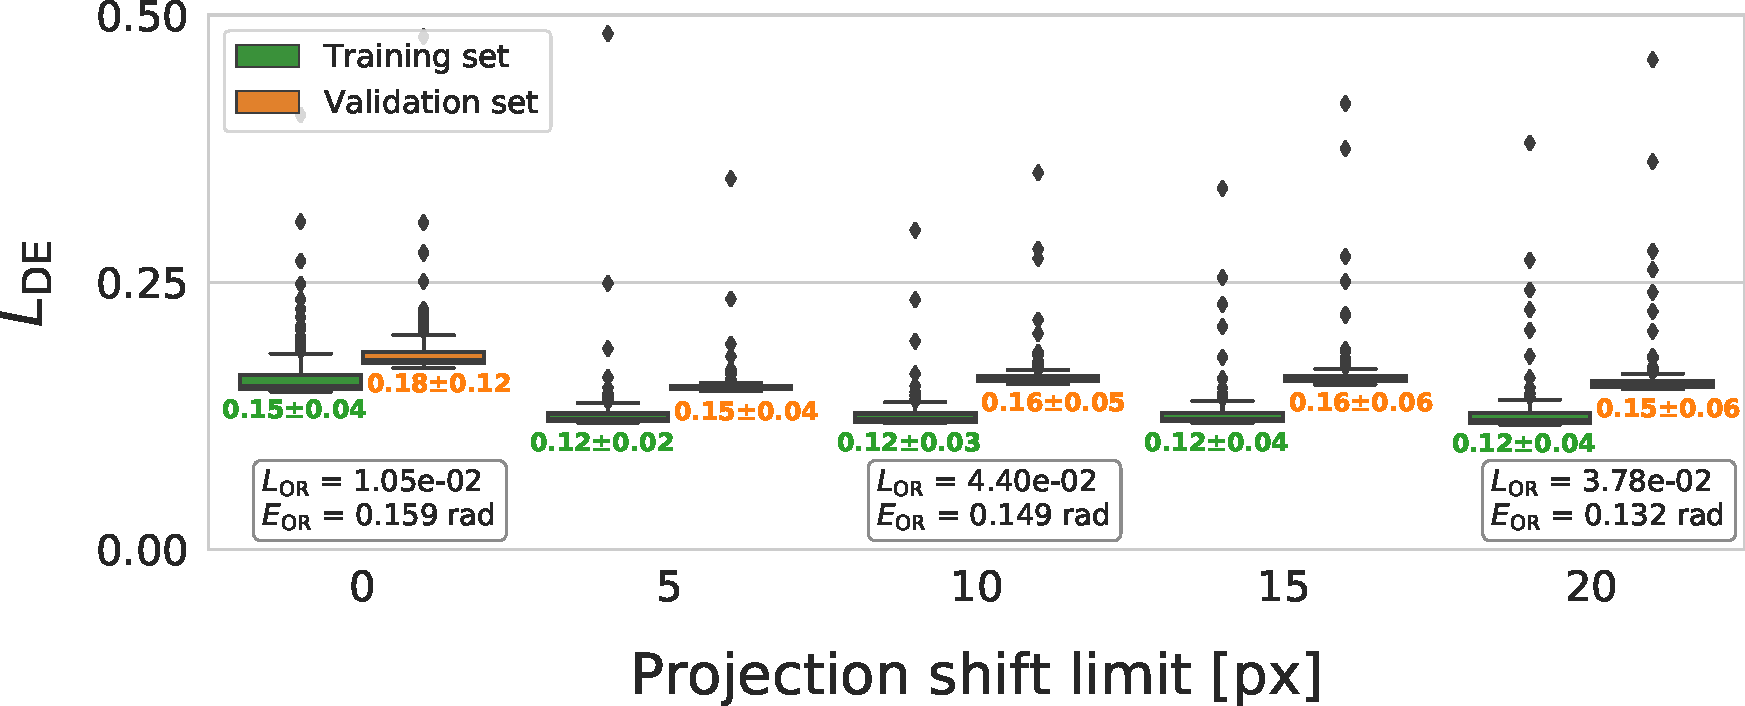
\includegraphics[height=5.5cm,valign=t]{figures/de_translation_nums}
        \caption{
        Variation of train and validation epoch losses w.r.t.\ projection translation of the asymmetric protein (\texttt{5j0n}). The mean orientation recovery error $E$ is in the red box, and the orientation recovery loss $OR$ is in the blue box.
        %\mdeff{We should try to have 12 and 13 side-by-side (to gain some space and facilitate comparison on the y-axis) by making them more square.}
    }\label{fig:distance-estimation-vary-projection-translation}
    \end{subfigure}
\end{figure}

\subsection*{Orientation recovery from estimated distances}

%\mdeff{Story: pipeline works but better distance estimation is needed for SOTA reconstruction.
%Method is however promising because learned distance is robust to perturbations and recovery works if distance works.}
%\todo{Justify threshold because of plateau (figref).
%Show recovered orientations w.r.t.\ ground truth after alignment.}
%\todo{Reconstruct the protein to show the full pipeline: from a set of projections to a reconstructed protein.
%Emphasize that it's a naive reconstruction algorithm.}

The orientation recovery from estimated distances represents a full pipeline needed to reconstruct the protein from a given set of projections.
We run the pipeline for both, asymmetric (\texttt{5j0n}) and symmetric (\texttt{5a1a}) protein.
In addition, we run the pipeline for the simulated realistic noise in the asymmetric protein.
The experimental setting for distance estimation is the similar to the one used to generate the \figref{learned-distance-siamese}: 150 epochs, 1e-3 learning rate, batch size 256 with random sampling of the projections, but for feature distance metric we use the geodesic distance since it showed the best performance in \figref{geo-eucl-mlp}.

Then, we run the orientation recovery on the estimated distances of the asymmetric protein and the performance results can be observed in \figref{5j0n-orientation-recovery-loss-est} with the same experimental setting as in \figref{5j0n-orientation-recovery-loss}.
With the noiseless projections, the objective function successfully converges to the $0.0510$ and with the noisy projections, the objective function converges to the $0.0683$.

\begin{figure}[ht!]
    \centering
    \begin{subfigure}[b]{0.45\textwidth}
        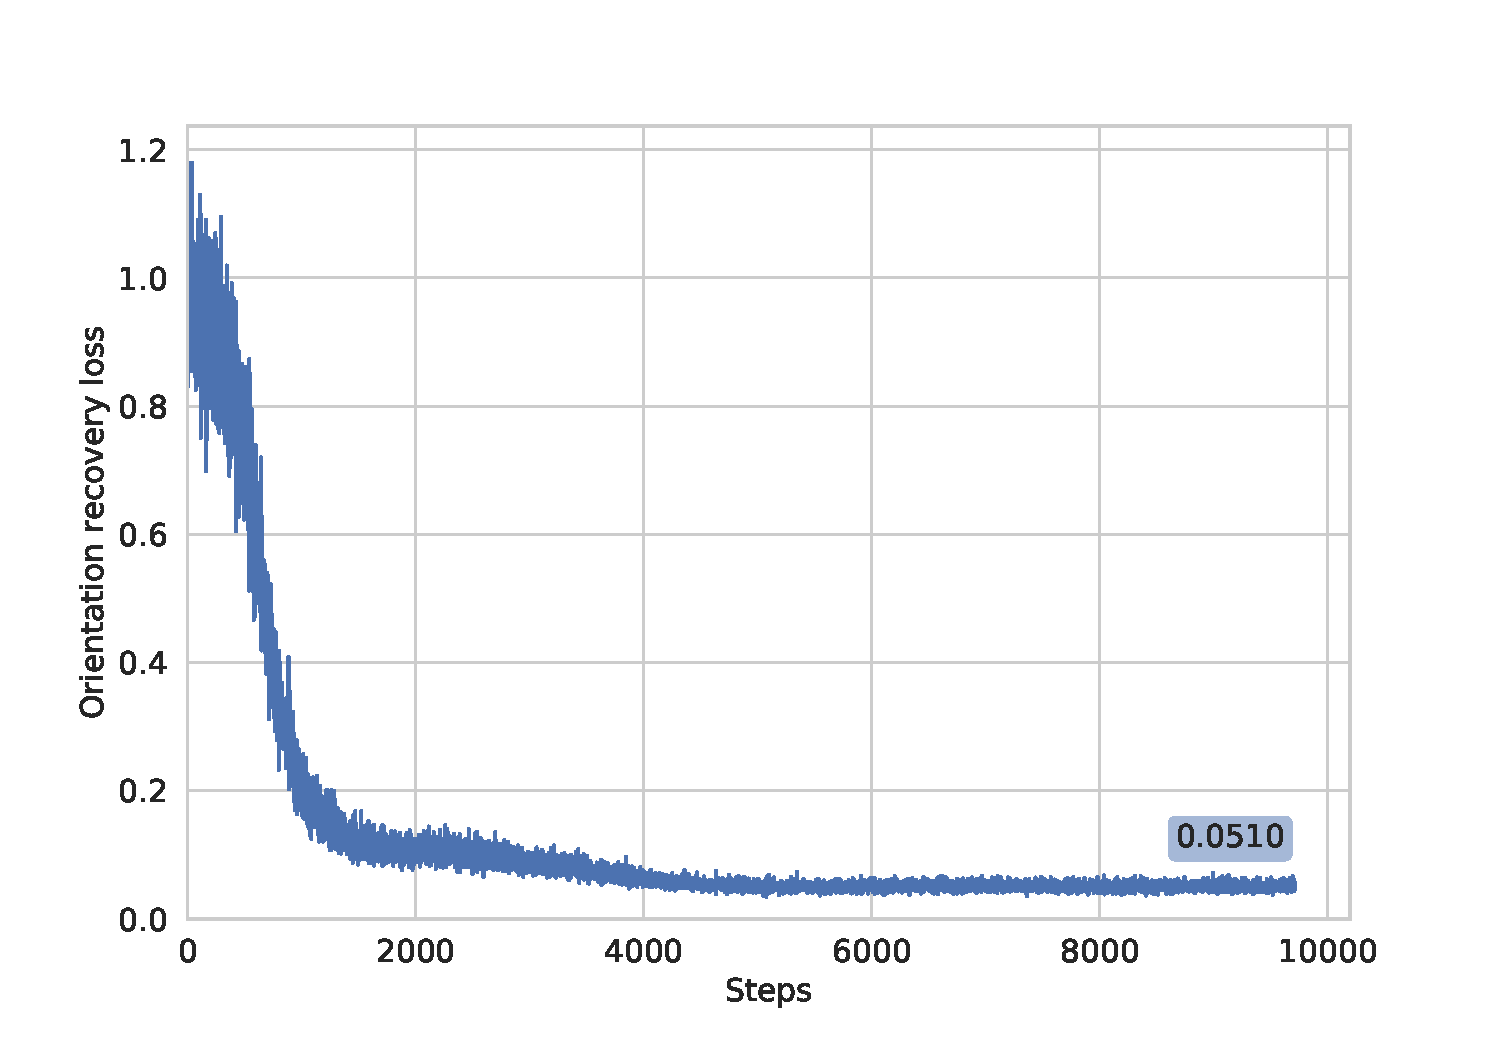
\includegraphics[height=5.5cm]{figures/5j0n_noise0_angle_recovery}
        \caption{Recovery loss, noiseless projections $\mathbf{Px}$.}
    \end{subfigure}
    \hfill
    \begin{subfigure}[b]{0.5\textwidth}
    \centering
        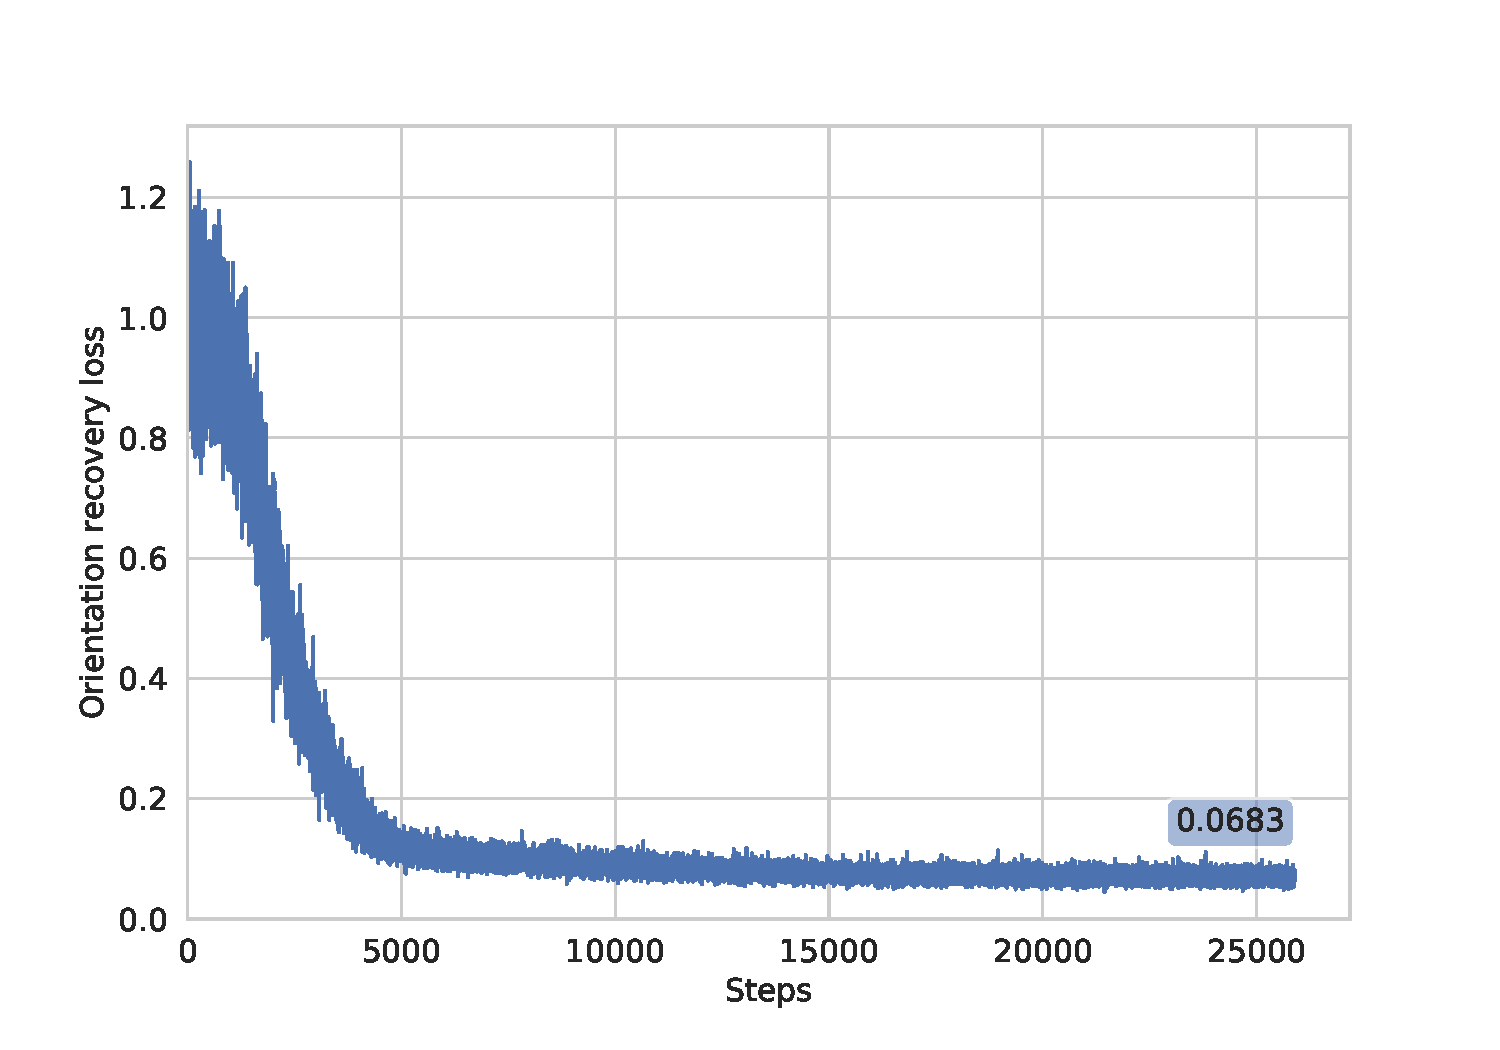
\includegraphics[height=5.5cm]{figures/5j0n_noise16_angle_recovery}
        \caption{Recovery loss, noisy projections $\mathbf{Px+n}, \; \mathbf{n} \sim \mathcal{N}(0, 16\mathbf{I})$.}
    \end{subfigure}
    \\
    \begin{subfigure}[b]{0.45\textwidth}
    \centering
        %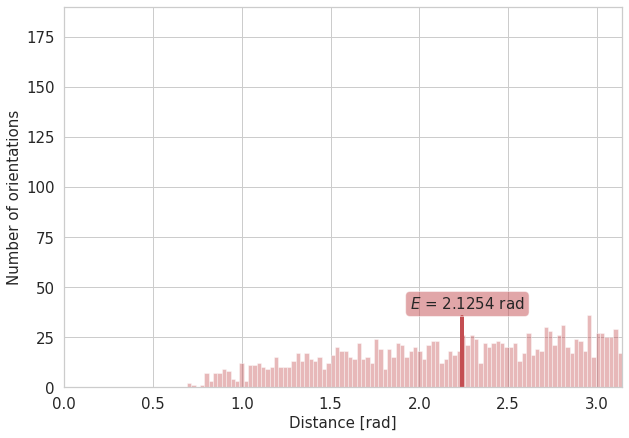
\includegraphics[height=5.7cm]{figures/5j0n_noise0_angle_alignment_before}
        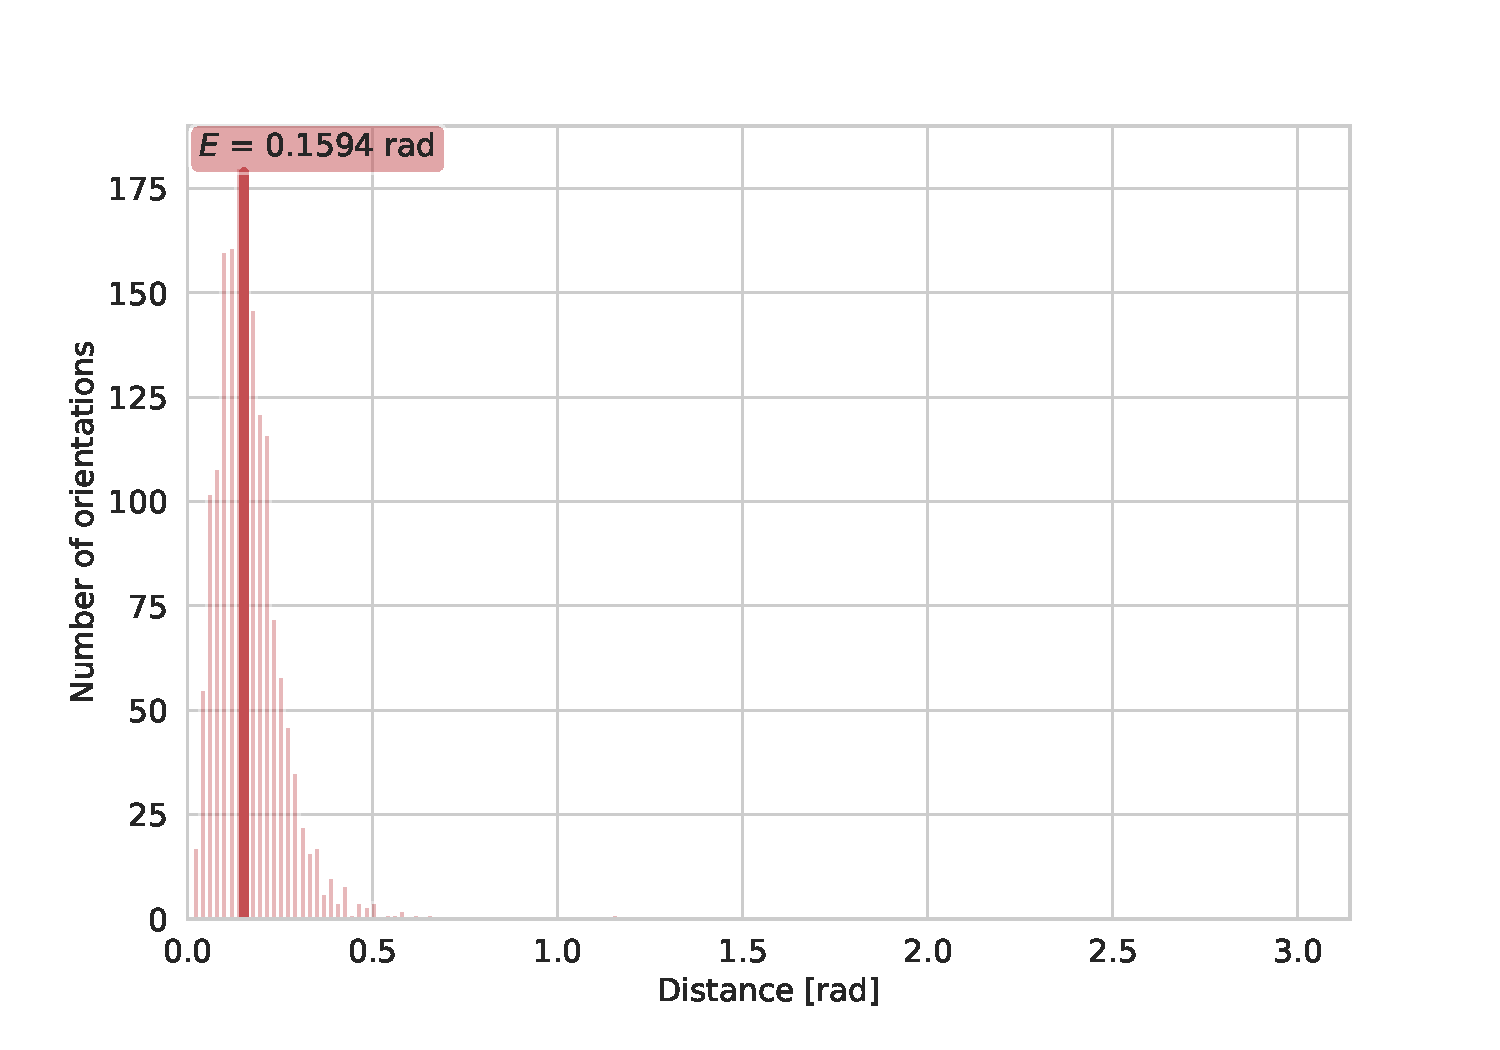
\includegraphics[height=5.7cm]{figures/5j0n_noise0_angle_alignment_after}
        \caption{Recovery error, noiseless projections $\mathbf{Px}$.}
        \label{fig:angle-alignment-5j0n-noise0}
    \end{subfigure}
    \hfill
    \begin{subfigure}[b]{0.5\textwidth}
    \centering
        %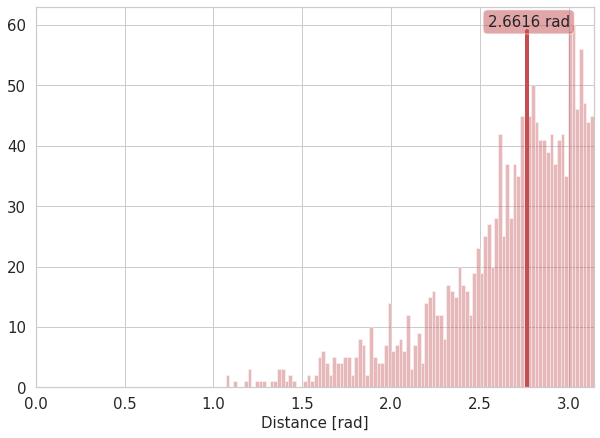
\includegraphics[height=5.7cm]{figures/5j0n_noise16_angle_alignment_before}
        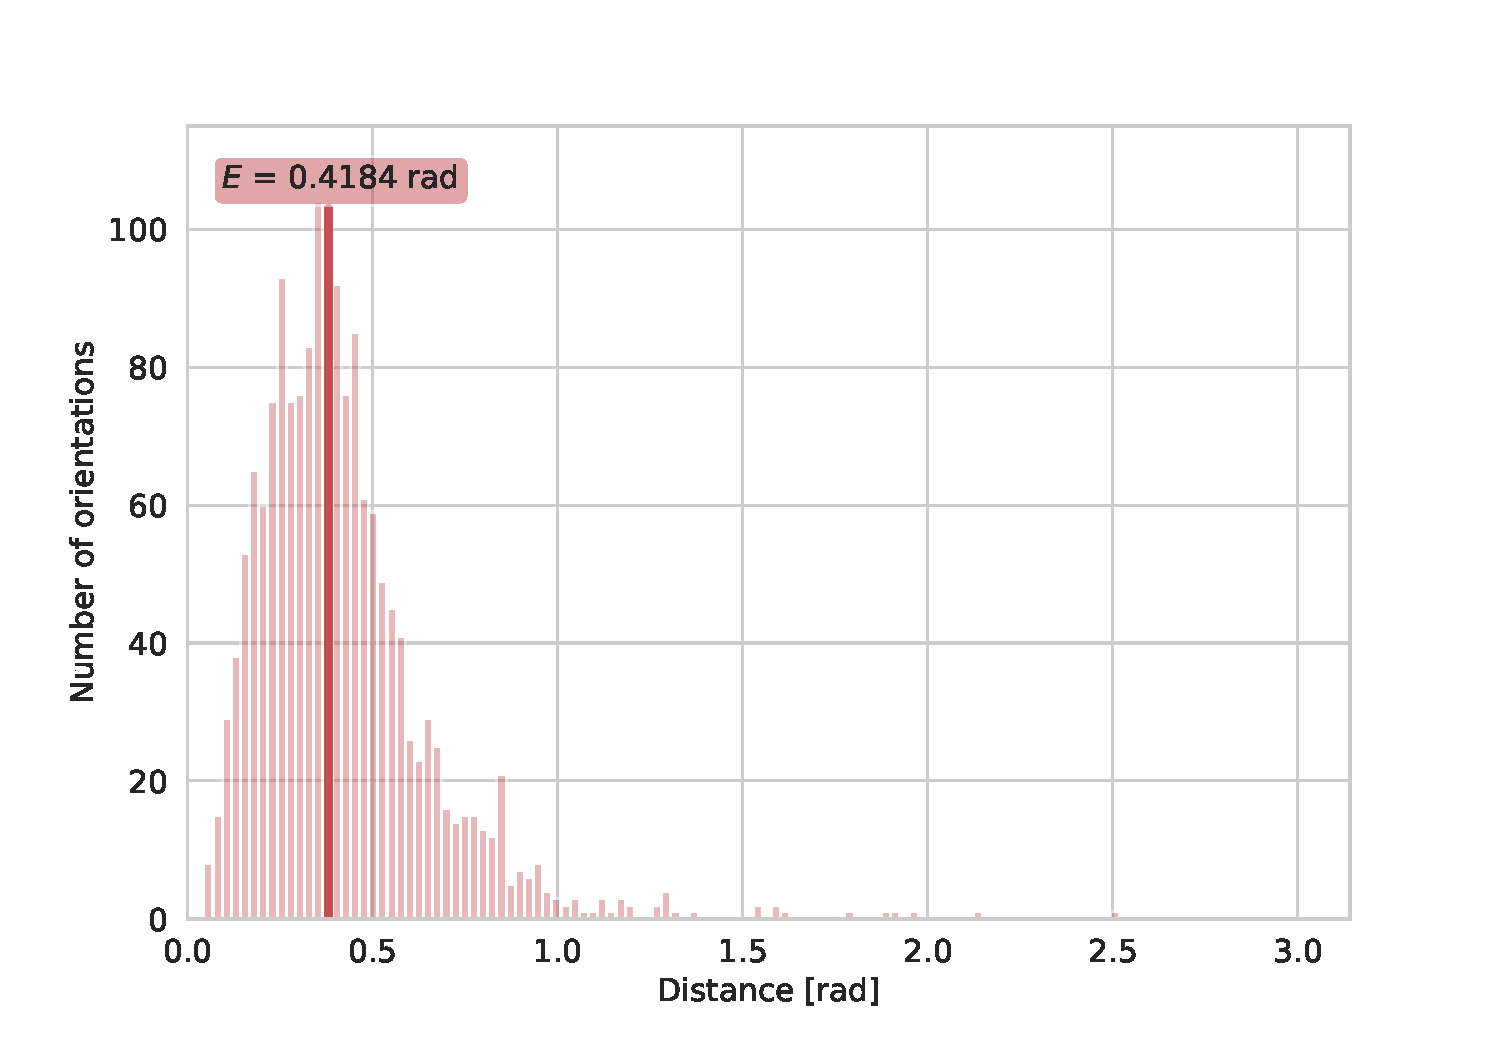
\includegraphics[height=5.7cm]{figures/5j0n_noise16_angle_alignment_after}
        \caption{Recovery error, noisy projections $\mathbf{Px+n}, \; \mathbf{n} \sim \mathcal{N}(0, 16\mathbf{I})$.}
        \label{fig:angle-alignment-5j0n-noise16}
    \end{subfigure}
    \caption{%
        Performance of orientation recovery of the asymmetric protein (\texttt{5j0n}) with (right) and without (left) noise.
        The first row shows the orientation recovery loss.
        The second row shows the orientation recovery error ($E$ from \eqnref{orientation-recovery-error}).
    }\label{fig:5j0n-orientation-recovery-loss-est}
\end{figure}

The mean orientation recovery error for asymmetric protein \texttt{5j0n} without noise in the projection can be seen in \figref{angle-alignment-5j0n-noise0}.
The smallest error achieved is $0.1594$ rad.
The mean orientation recovery error for asymmetric protein \texttt{5j0n} with noisy projections (white noise with variance 16) can be seen in \figref{angle-alignment-5j0n-noise16}.
The smallest error achieved is $0.4184$ rad.

As a last step of the pipeline, we perform protein reconstruction using the projections and their corresponding estimated orientations.
For that, we again use the ASTRA toolbox.
Using this toolbox, we generate orientation vectors based on angles which we later feed into projection 3D geometry in ASTRA.
Due to GPU memory limit, we are able to reconstruct the protein using maximum of $3,000$ projections.
It holds for our case, since we perform orientation recovery on the test set which has in total $1,650$ projections (less than the limit of $3,000$).

The reconstruction results for the asymmetric protein (\texttt{5j0n}) with noiseless projections can be seen in \figref{5j0n-reconstruction-noise0}. On the left side we have a reconstruction using the ground-truth orientations, and on the right side we have the reconstruction result using the estimated aligned orientations.

\begin{figure}[ht!]
    \centering
    \begin{subfigure}[b]{0.49\linewidth}
        \centering
        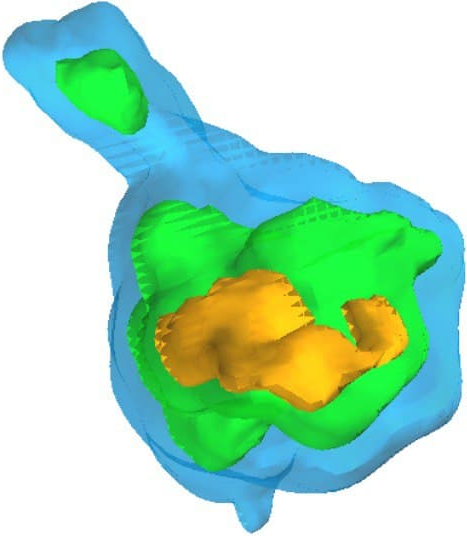
\includegraphics[width=0.90\linewidth]{figures/5j0n_reconstruction_GT}
        \caption{Noiseless projections $\mathbf{Px}$, true orientations ${\big\{q_p\big\}}_{p=1}^P$.}
    \end{subfigure}
    \hfill
    \begin{subfigure}[b]{0.49\linewidth}
        \centering
        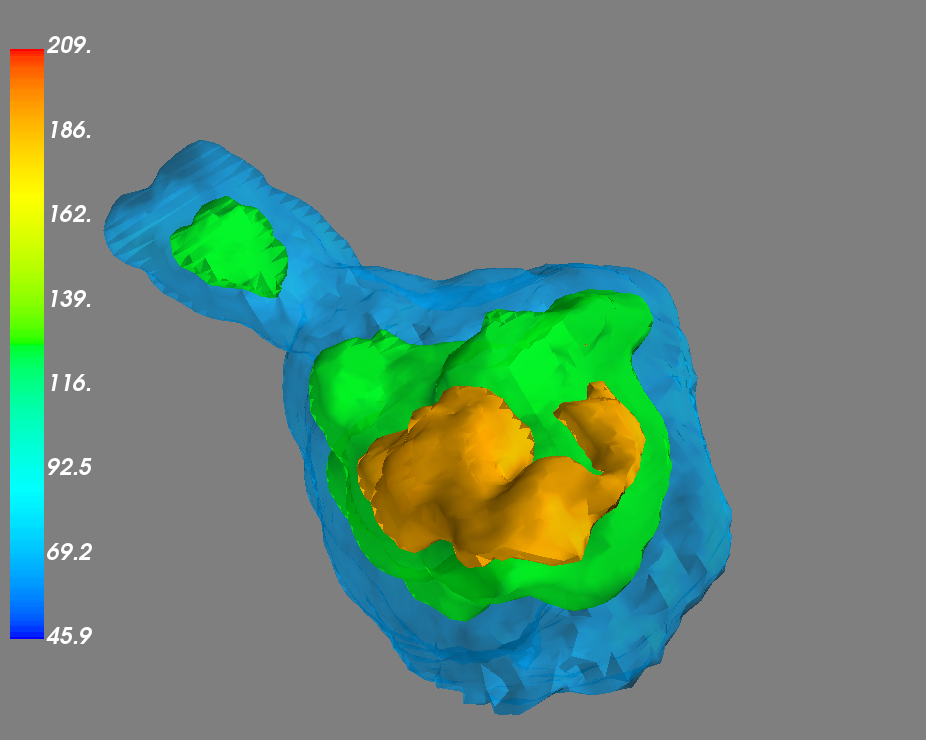
\includegraphics[width=0.90\linewidth]{figures/5j0n_reconstruction_GT_noise16}
        \caption{Noisy projections $\mathbf{Px + n}$, true orientations ${\big\{q_p\big\}}_{p=1}^P$.}
    \end{subfigure}
    \\
    \begin{subfigure}[b]{0.49\linewidth}
        \centering
        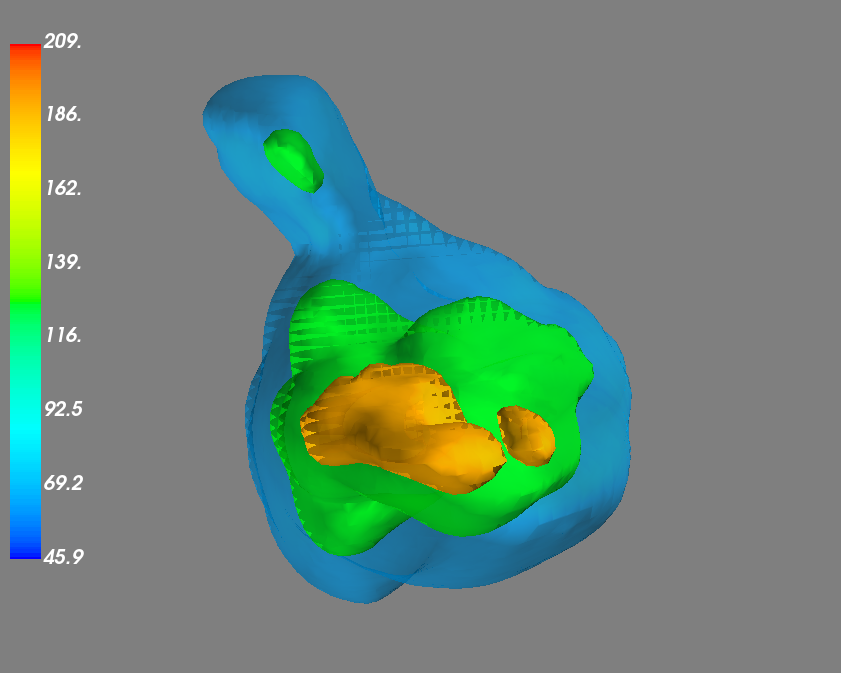
\includegraphics[width=0.90\linewidth]{figures/5j0n_reconstruction_noise0}
        \caption{Noiseless projections $\mathbf{Px}$, recovered orientations ${\big\{\widehat{q_p}\big\}}_{p=1}^P$.}
    \end{subfigure}
    \hfill
    \begin{subfigure}[b]{0.49\linewidth}
        \centering
        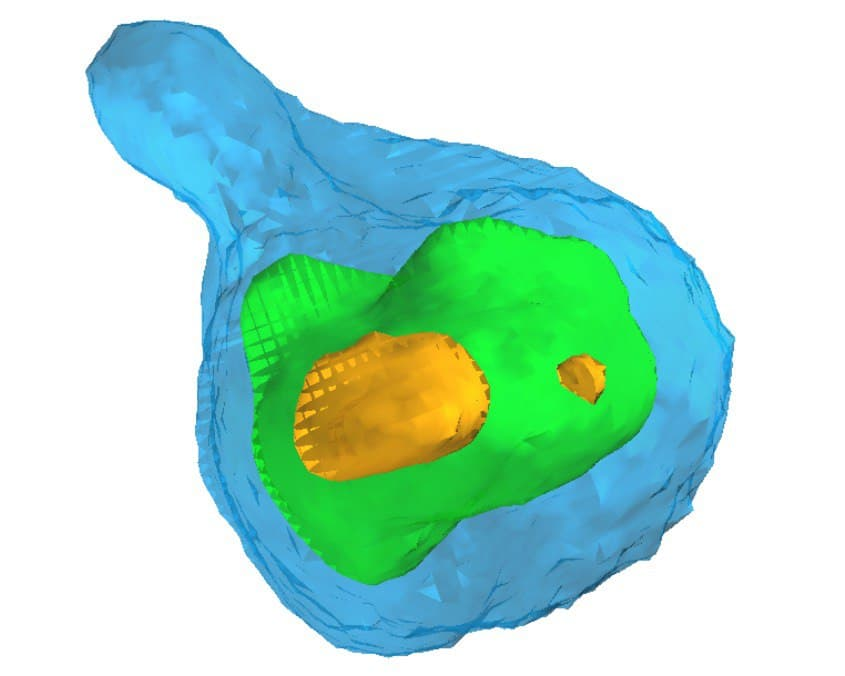
\includegraphics[width=0.90\linewidth]{figures/5j0n_reconstruction_noise16}
        \caption{Noisy projections $\mathbf{Px + n}$, recovered orientations ${\big\{\widehat{q_p}\big\}}_{p=1}^P$.}
    \end{subfigure}
    \caption{
        Performance of orientation recovery of the asymmetric protein (\texttt{5j0n}) with (right) and without (left) noise.
        Reconstruction of the asymmetric protein (\texttt{5j0n}) from noiseless (left) and noisy (right) projections ${\big\{\p_i\big\}}_{i=1}^P$ and true (top) and recovered (bottom) orientations.
    }\label{fig:5j0n-reconstruction-noise0}
    \label{fig:5j0n-reconstruction-noise16}
\end{figure}

The reconstruction results for the asymmetric protein (\texttt{5j0n}) with noisy projections (with noise variance 16) can be seen in \figref{5j0n-reconstruction-noise16}.
Similarly, on the left side we have a reconstruction using the ground-truth orientations, and on the right side we have the reconstruction result using the estimated aligned orientations.

Similarly, we run the whole reconstruction pipeline on the symmetric protein (\texttt{5a1a}).
The experimental conditions for the distance estimation are the same as for the asymmetric protein, except that we use the quarter-sphere projections coverage (whereas, in the asymmetric protein we use half-sphere coverage).
The orientation recovery loss can be seen in \figref{5a1a-orientation-recovery-loss}. It successfully converges to $0.0381$.
The mean orientation recovery error for symmetric protein \texttt{5a1a} can be seen in \figref{angle-alignment-5a1a-noise0}. The smallest error achieved is $0.1871$ rad.

\begin{figure}[ht!]
    \centering
    \begin{subfigure}[b]{0.45\textwidth}
        \centering
        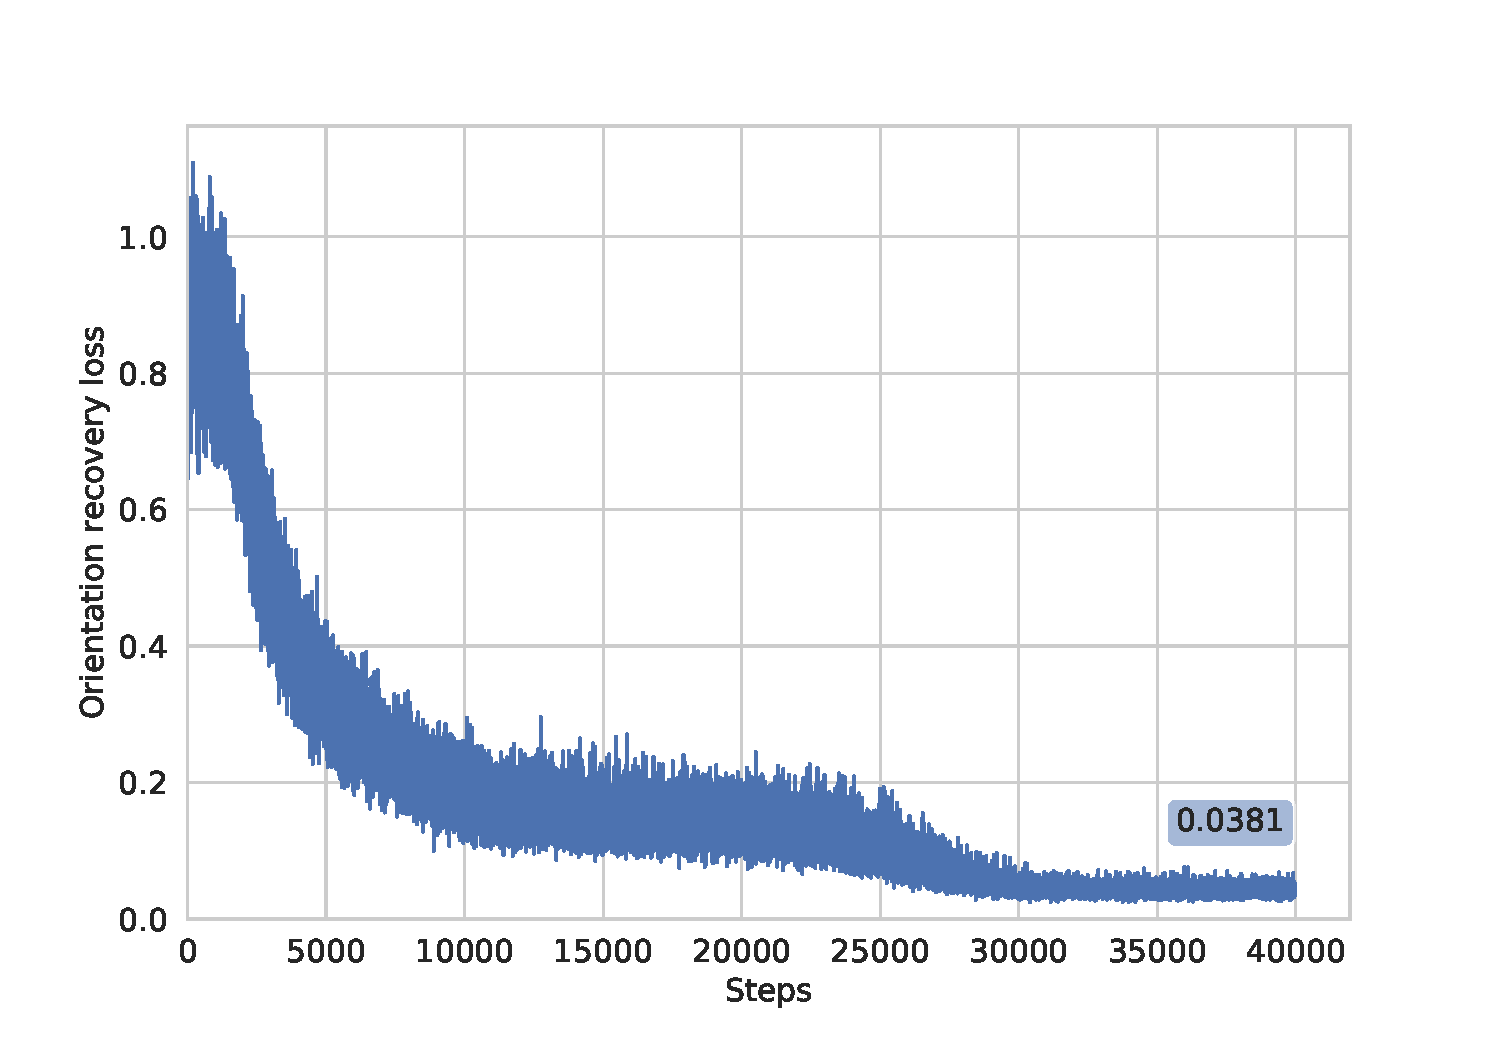
\includegraphics[height=5.5cm]{figures/5a1a_noise0_angle_recovery}
        \caption{Orientation recovery loss \eqnref{orientation-recovery}.}
    \end{subfigure}
    \hfill
    \begin{subfigure}[b]{0.45\textwidth}
        \centering
        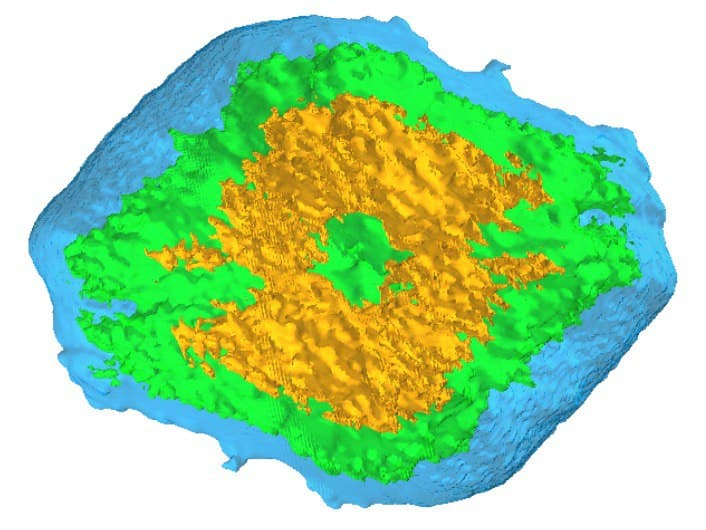
\includegraphics[height=5.5cm]{figures/5a1a_ground_truth}
        \caption{Reconstruction from true orientations ${\big\{q_p\big\}}_{p=1}^P$.}
    \end{subfigure}
    \\
    \begin{subfigure}[b]{0.45\textwidth}
        \centering
        %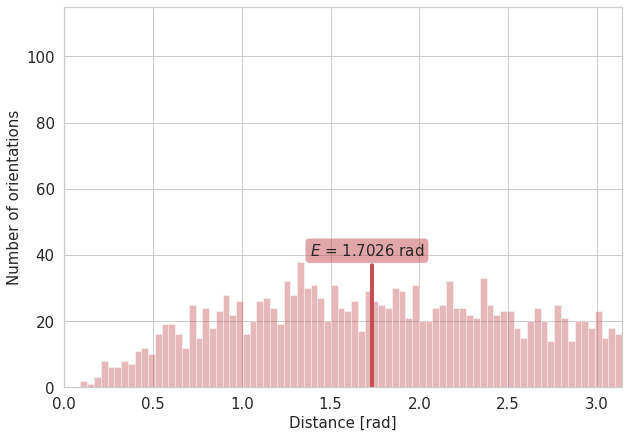
\includegraphics[height=5.7cm]{figures/5a1a_noise0_angle_alignment_before}
        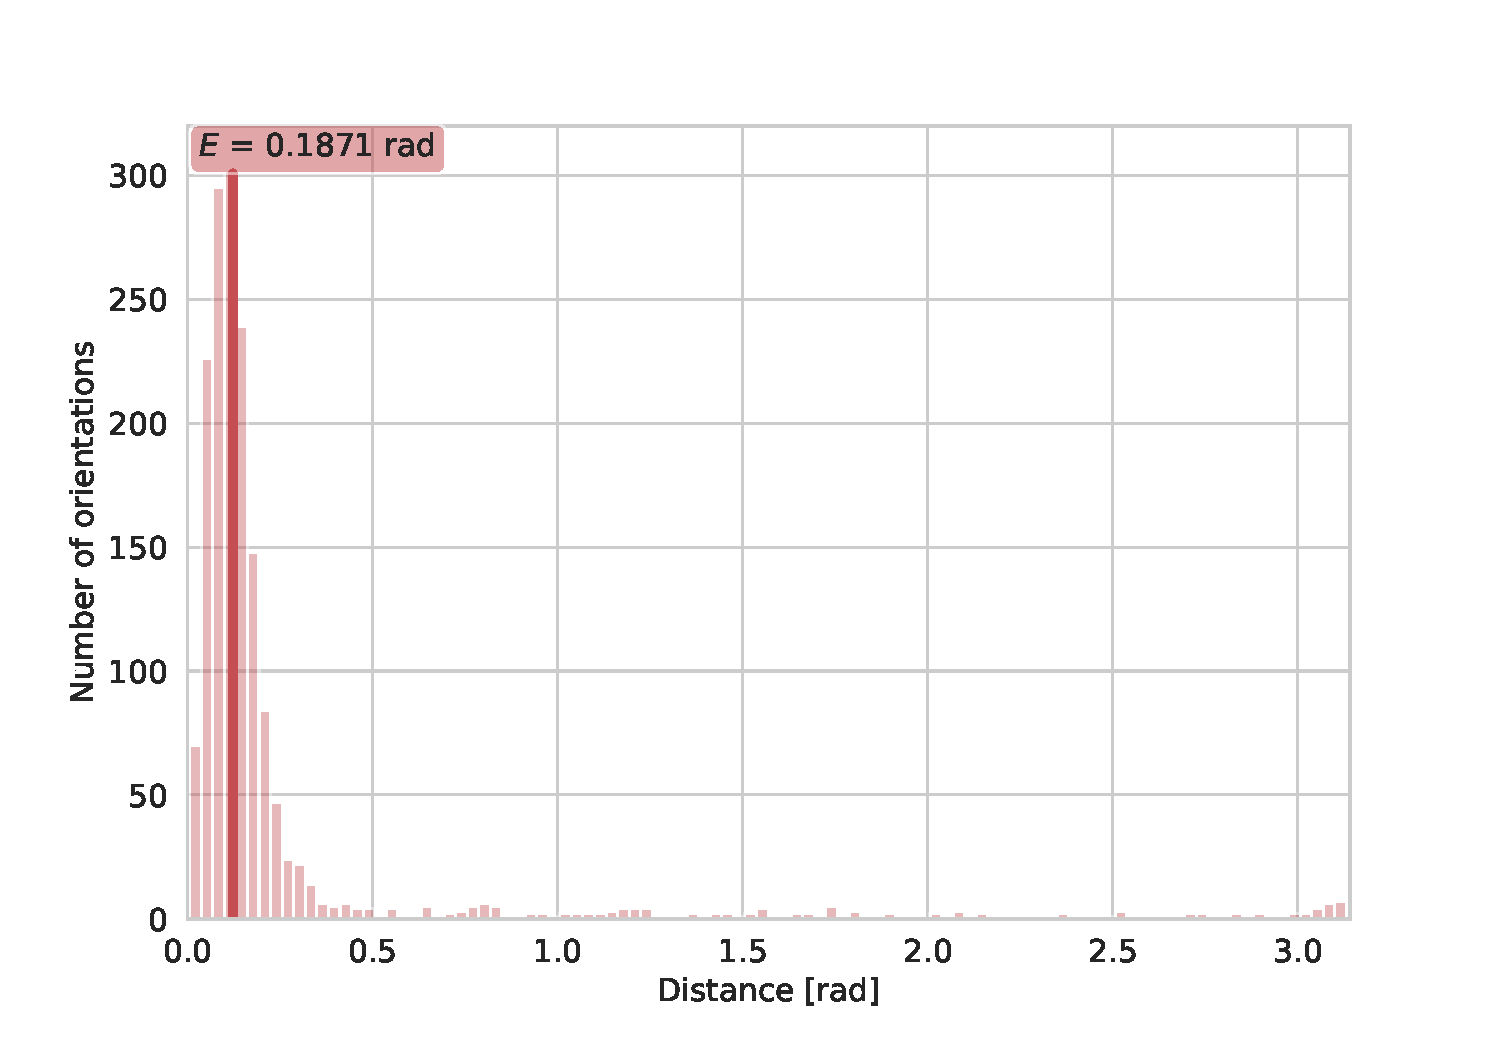
\includegraphics[height=5.5cm]{figures/5a1a_noise0_angle_alignment_after}
        \caption{Orientation recovery error \eqnref{orientation-recovery-error}.}
    \end{subfigure}
    \hfill
    \begin{subfigure}[b]{0.45\textwidth}
        \centering
        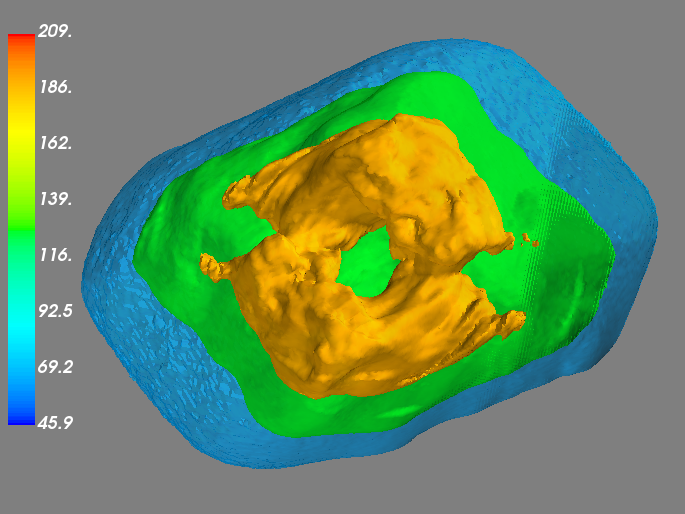
\includegraphics[height=5.5cm]{figures/5a1a_aligned}
        \caption{Reconstruction from recovered orientations ${\big\{\widehat{q_p}\big\}}_{p=1}^P$.}
    \end{subfigure}
    \caption{
        Orientation recovery and reconstruction of the symmetric protein (\texttt{5a1a}) from noiseless projections.
    }\label{fig:5a1a-orientation-recovery-loss}
    \label{fig:angle-alignment-5a1a-noise0}
    \label{fig:5a1a-reconstruction-noise0}
\end{figure}

Lastly, we perform the protein reconstruction with the same ASTRA toolbox setting as for the asymmetric protein. The results of the reconstruction can be observed in the \figref{5a1a-reconstruction-noise0}.
We were able to successfully reconstruct the symmetric protein even though the distance estimation was noisier than the one performed on the asymmetric protein.

We observe that the pipeline works, but for the state-of-the-art reconstruction we need a better distance estimation.
However, the method developed is promising since the learned distance is robust to perturbations.
We observe that the orientation recovery and distance estimation are interconnected, \textit{i.e.} if one works the other one will work.

To check the generalization to unseen proteins, and not only to  unseen projections, we train the distance estimation on the set of four different proteins (\texttt{5nvu}~\cite{5nvu_pdb}, \texttt{5nvs}~\cite{5nvs_pdb}, \texttt{6mem}~\cite{6mem_pdb}, \texttt{6o1o}~\cite{6o1o_pdb}) that have the same type of symmetry (asymmetric  C1) as the one protein (\texttt{5j0n}) in the test dataset that is used in orientation recovery.
The orientation recovery reaches the error of 0.0352.
This proves that distance learning is able to abstract the protein and that way generalize the distance metric to the unseen proteins.
